
% *************** LEd - dokument oparty na szablonie pracy magisterskiej ***************

\documentclass[12pt,apalike,a4paper,openright,twoside,makeidx]{memoir}
% *************** Definicje stylu dokumentu ***************

% *********************************************************************************
% W piku tym zdefiniowany jest wygl�d dokumentu.
% Zmiany tutaj nie s� konieczne o ile nie zamierzasz zmienia� wygl�du dokumentu.
% *********************************************************************************

% *************** Za�adowanie pakiet�w ***************




\usepackage{graphicx}
\usepackage{float}
\usepackage{epsfig}
\usepackage{amsmath}
\usepackage{amssymb}
\usepackage{amsthm}
\usepackage{booktabs}
\usepackage{stmaryrd}
\usepackage{url}
\usepackage{longtable}

\usepackage{polski}
%\usepackage{indentfirst}
\usepackage[cp1250]{inputenc}


\usepackage{listings}
\usepackage{amsmath}
\usepackage{amsfonts}
\usepackage{amssymb}
\usepackage{amsthm}
\usepackage{bookman}


%\renewcommand*{\lstlistingname}{Spis listing�w kodu}


%\renewcommand{\bf}{\textbf}












% *************** W��czenie tworzenia skorowidza ***************
\makeindex

% *************** Dodanie do pozycji bibliograficznych informacji o numerze strony, na kt�rej jest ona cytowana ***************
\usepackage{citeref}
\renewcommand{\bibitempages}[1]{\newblock {\scriptsize }}

% *************** Definicje niekt�rych kolor�w ***************
\usepackage{color}

\definecolor{greenyellow}   {cmyk}{0.15, 0   , 0.69, 0   }
\definecolor{yellow}        {cmyk}{0   , 0   , 1   , 0   }
\definecolor{goldenrod}     {cmyk}{0   , 0.10, 0.84, 0   }
\definecolor{dandelion}     {cmyk}{0   , 0.29, 0.84, 0   }
\definecolor{apricot}       {cmyk}{0   , 0.32, 0.52, 0   }
\definecolor{peach}         {cmyk}{0   , 0.50, 0.70, 0   }
\definecolor{melon}         {cmyk}{0   , 0.46, 0.50, 0   }
\definecolor{yelloworange}  {cmyk}{0   , 0.42, 1   , 0   }
\definecolor{orange}        {cmyk}{0   , 0.61, 0.87, 0   }
\definecolor{burntorange}   {cmyk}{0   , 0.51, 1   , 0   }
\definecolor{bittersweet}   {cmyk}{0   , 0.75, 1   , 0.24}
\definecolor{redorange}     {cmyk}{0   , 0.77, 0.87, 0   }
\definecolor{mahogany}      {cmyk}{0   , 0.85, 0.87, 0.35}
\definecolor{maroon}        {cmyk}{0   , 0.87, 0.68, 0.32}
\definecolor{brickred}      {cmyk}{0   , 0.89, 0.94, 0.28}
\definecolor{red}           {cmyk}{0   , 1   , 1   , 0   }
\definecolor{orangered}     {cmyk}{0   , 1   , 0.50, 0   }
\definecolor{rubinered}     {cmyk}{0   , 1   , 0.13, 0   }
\definecolor{wildstrawberry}{cmyk}{0   , 0.96, 0.39, 0   }
\definecolor{salmon}        {cmyk}{0   , 0.53, 0.38, 0   }
\definecolor{carnationpink} {cmyk}{0   , 0.63, 0   , 0   }
\definecolor{magenta}       {cmyk}{0   , 1   , 0   , 0   }
\definecolor{violetred}     {cmyk}{0   , 0.81, 0   , 0   }
\definecolor{rhodamine}     {cmyk}{0   , 0.82, 0   , 0   }
\definecolor{mulberry}      {cmyk}{0.34, 0.90, 0   , 0.02}
\definecolor{redviolet}     {cmyk}{0.07, 0.90, 0   , 0.34}
\definecolor{fuchsia}       {cmyk}{0.47, 0.91, 0   , 0.08}
\definecolor{lavender}      {cmyk}{0   , 0.48, 0   , 0   }
\definecolor{thistle}       {cmyk}{0.12, 0.59, 0   , 0   }
\definecolor{orchid}        {cmyk}{0.32, 0.64, 0   , 0   }
\definecolor{darkorchid}    {cmyk}{0.40, 0.80, 0.20, 0   }
\definecolor{purple}        {cmyk}{0.45, 0.86, 0   , 0   }
\definecolor{plum}          {cmyk}{0.50, 1   , 0   , 0   }
\definecolor{violet}        {cmyk}{0.79, 0.88, 0   , 0   }
\definecolor{royalpurple}   {cmyk}{0.75, 0.90, 0   , 0   }
\definecolor{blueviolet}    {cmyk}{0.86, 0.91, 0   , 0.04}
\definecolor{periwinkle}    {cmyk}{0.57, 0.55, 0   , 0   }
\definecolor{cadetblue}     {cmyk}{0.62, 0.57, 0.23, 0   }
\definecolor{cornflowerblue}{cmyk}{0.65, 0.13, 0   , 0   }
\definecolor{midnightblue}  {cmyk}{0.98, 0.13, 0   , 0.43}
\definecolor{navyblue}      {cmyk}{0.94, 0.54, 0   , 0   }
\definecolor{royalblue}     {cmyk}{1   , 0.50, 0   , 0   }
\definecolor{blue}          {cmyk}{1   , 1   , 0   , 0   }
\definecolor{cerulean}      {cmyk}{0.94, 0.11, 0   , 0   }
\definecolor{cyan}          {cmyk}{1   , 0   , 0   , 0   }
\definecolor{processblue}   {cmyk}{0.96, 0   , 0   , 0   }
\definecolor{skyblue}       {cmyk}{0.62, 0   , 0.12, 0   }
\definecolor{turquoise}     {cmyk}{0.85, 0   , 0.20, 0   }
\definecolor{tealblue}      {cmyk}{0.86, 0   , 0.34, 0.02}
\definecolor{aquamarine}    {cmyk}{0.82, 0   , 0.30, 0   }
\definecolor{bluegreen}     {cmyk}{0.85, 0   , 0.33, 0   }
\definecolor{emerald}       {cmyk}{1   , 0   , 0.50, 0   }
\definecolor{junglegreen}   {cmyk}{0.99, 0   , 0.52, 0   }
\definecolor{seagreen}      {cmyk}{0.69, 0   , 0.50, 0   }
\definecolor{green}         {cmyk}{1   , 0   , 1   , 0   }
\definecolor{forestgreen}   {cmyk}{0.91, 0   , 0.88, 0.12}
\definecolor{pinegreen}     {cmyk}{0.92, 0   , 0.59, 0.25}
\definecolor{limegreen}     {cmyk}{0.50, 0   , 1   , 0   }
\definecolor{yellowgreen}   {cmyk}{0.44, 0   , 0.74, 0   }
\definecolor{springgreen}   {cmyk}{0.26, 0   , 0.76, 0   }
\definecolor{olivegreen}    {cmyk}{0.64, 0   , 0.95, 0.40}
\definecolor{rawsienna}     {cmyk}{0   , 0.72, 1   , 0.45}
\definecolor{sepia}         {cmyk}{0   , 0.83, 1   , 0.70}
\definecolor{brown}         {cmyk}{0   , 0.81, 1   , 0.60}
\definecolor{tan}           {cmyk}{0.14, 0.42, 0.56, 0   }
\definecolor{gray}          {cmyk}{0   , 0   , 0   , 0.50}
\definecolor{black}         {cmyk}{0   , 0   , 0   , 1   }
\definecolor{white}         {cmyk}{0   , 0   , 0   , 0   } 

% *************** W��czenie hyperlink�w w dokumentach PDF ***************
\ifpdf
    \pdfcompresslevel=9
        \usepackage[plainpages=false,pdfpagelabels,bookmarksnumbered,%
        colorlinks=false,%
        linkcolor=sepia,%
        citecolor=sepia,%
        filecolor=maroon,%
        pagecolor=red,%
        urlcolor=sepia,%
        pdftex,%
        unicode]{hyperref} 
    \input supp-mis.tex
    \input supp-pdf.tex
    \pdfimageresolution=600
    \usepackage{thumbpdf} 
\else
    \usepackage{hyperref}
\fi

\usepackage{memhfixc}

% *************** Wygl�d strony marginesy ***************
\settypeblocksize{*}{32pc}{1.618}
%Rozne marginesy
%\textwidth=16cm
%\setlrmargins{*}{20mm}{*}
%\setulmargins{*}{*}{1.3}

%Takie same
\setlrmargins{*}{1.47in}{*}
\setulmargins{*}{*}{1.3}

\setheadfoot{\onelineskip}{2\onelineskip}
\setheaderspaces{*}{2\onelineskip}{*}

\def\baselinestretch{1.1}

\checkandfixthelayout


% *************** Stylu rozdzia��w i podrozdzia��w ***************
\makechapterstyle{mychapterstyle}{%
    \renewcommand{\chapnamefont}{\LARGE\sffamily\bfseries}%
    \renewcommand{\chapnumfont}{\LARGE\sffamily\bfseries}%
    \renewcommand{\chaptitlefont}{\Huge\sffamily\bfseries}%
    \renewcommand{\printchaptertitle}[1]{%
        \chaptitlefont\hrule height 0.5pt \vspace{1em}%
        {##1}\vspace{1em}\hrule height 0.5pt%
        }%
    \renewcommand{\printchapternum}{%
        \chapnumfont\thechapter%
        }%
}

\chapterstyle{mychapterstyle}

\setsecheadstyle{\Large\sffamily\bfseries}
\setsubsecheadstyle{\large\sffamily\bfseries}
\setsubsubsecheadstyle{\normalfont\sffamily\bfseries}
\setparaheadstyle{\normalfont\sffamily}

\makeevenhead{headings}{\thepage}{}{\small\slshape\leftmark}
\makeoddhead{headings}{\small\slshape\rightmark}{}{\thepage}

% *************** Styl spisu tre�ci ***************
\settocdepth{subsection}

\setsecnumdepth{subsection}
\maxsecnumdepth{subsection}
\settocdepth{subsection}
\maxtocdepth{subsection}

% ********** Polecenia do mott **********
\setlength{\epigraphwidth}{0.57\textwidth}
\setlength{\epigraphrule}{0pt}
\setlength{\beforeepigraphskip}{1\baselineskip}
\setlength{\afterepigraphskip}{2\baselineskip}

\newcommand{\epitext}{\sffamily\itshape}
\newcommand{\epiauthor}{\sffamily\scshape ---~}
\newcommand{\epititle}{\sffamily\itshape}
\newcommand{\epidate}{\sffamily\scshape}
\newcommand{\episkip}{\medskip}

\newcommand{\myepigraph}[4]{%
	\epigraph{\epitext #1\episkip}{\epiauthor #2\\\epititle #3 \epidate(#4)}\noindent}

% *************** Inne ***************
\renewcommand{\thefootnote}{\fnsymbol{footnote}}

\DeclareGraphicsExtensions{.png, .bb}


% *************** Koniec definicji stylu dokumentu ***************



\begin{document}
% *************** Front matter ***************
\frontmatter
%% *************** Front matter ***************

% ************************************************************
% W tym miejscu mo�esz zdefiniowa� wygl�d strony tytu�owej
% Mo�esz tak�e zdefiniowa� dedykacj� albo wy��czy� j�
% ************************************************************

% *************** Strona tytu�owa ***************
\pagestyle{empty}
\sffamily

\linespread{1.0}
\noindent

% \begin{figure}
%	\centering
%		
\includegraphics[width=1.0\textwidth]{logo.pdf}
%	\label{fig:logo}
% \end{figure}

\vfill\vfill
\begin{center}
    \Large\bfseries
    PRACA DYPLOMOWA - IN�YNIERSKA\\
\end{center}

\vfill
\begin{center}
    \Large
    Konrad Rodzik\\
    nr albumu: 215039
\end{center}

\vfill
\begin{center}
    \Large\bfseries
    NVIDIA CUDA jako technologia przy�pieszaj�ca metode �ledzenia promieni
\end{center}

\vfill\vfill\vfill
\begin{flushright}
    \Large
    Kierownik pracy:\\ Prof. nazw. dr hab. in�. Dariusz Sawicki
\end{flushright}
\vfill

\begin{flushleft}
....................................................\\
\ \ ocena pracy \\
\vfill
....................................................\\
\ \ data i podpis Przewodnicz�cego\\
\ \ Komisji Egzaminacyjnej Dyplomowego
\end{flushleft}

\vfill
\begin{center}
\large
    Warszawa, 2011
\end{center}


\chapter*{�yciorys}
Urodzi�em si�  1 listopada 1987 r.  w Radomiu w rodzinie inteligenckiej. Ojciec in�ynier, matka z wykszta�cenia prawnik.
W roku 2003 uko�czy�em gimnazjum i rozpocz��em nauk� w VI Liceum Og�lnokszta�c�cym im. J. Kochanowskiego w Radomiu w klasie o profilu matematyczno-fizyczno-informatycznym. 
Po maturze w roku 2006 zosta�em studentem na Wydziale Elektroniki i Technik Informacyjnych Politechniki Warszawskiej na kierunku Telekomunikacja.  

Od 2008 r. jestem cz�onkiem ko�a naukowego  "Brama". Zajmuj� si� badaniami i rozwojem system�w i aplikacji mobilnych. 
Interesuj� si� systemami oraz aplikacjami mobilnymi oraz mechanizmami wspierania proces�w nauki i zapami�tywania. 

Moje zainteresowania to: bieganie, sporty walki oraz windsurfing.

\cleardoublepage

\begin{abstract}
\noindent \textbf{Tytu�:  Mobilny system dobierania kierowc�w i pasa�er�w do wsp�lnej podr�y: "mobiStopowicz"}\\
Niniejsza praca in�ynierska opisuje projekt mobilnego systemu przeznaczonego dla kierowc�w i podr�nych, kt�rego celem jest wspieranie procesu dobierania si� do wsp�lnej podr�y. W pracy przeprowadzi�em wst�pn� analiz� sytuacji na rynku, opracowa�em algorytm parowania oraz zaprojektowa�em architektur� systemu. Nast�pnie zosta� opisany projekt, implementacja oraz perspektywa wdro�enia systemu.\\\\\\


\begin{center}\textbf{Abstract}\end{center}
\textbf{Title: Mobile system designed for pairing divers and travelers to collective travel: "mobiStopowicz"}\\
The bachelor thesis describes the mobile system aimed at pairing drivers and travelers to collective travel. In the thesis I have analyzed state of the art. Then pairing algorithm and architecture of the system was designed. The thesis also describes project, implementation and deployment opportunities of the mobiStopowicz system.

\end{abstract}

\clearpage

\rmfamily
\normalfont
% *************** Spis tre�ci ***************
\pagenumbering{roman}
\pagestyle{headings}
\tableofcontents

% *************** Koniec front matter ***************

% *************** Spis tre�ci ***************
\pagenumbering{roman}
\pagestyle{headings}
\tableofcontents
















\definecolor{ListingBackground}{rgb}{0.95,0.95,0.95}


\lstdefinestyle{outcode}
{
basicstyle={\footnotesize},
keywordstyle=\color[rgb]{0,0,1}, 
commentstyle=\color[rgb]{0.133,0.545,0.133}, 
stringstyle=\color[rgb]{0.627,0.126,0.941}, 
numbers=left, 
stepnumber=1, 
firstnumber=1,
numberfirstline=true,
numberblanklines=false, 
numbersep=10pt, 
tabsize=2,
xleftmargin=17pt,
framexleftmargin=3pt,
framexbottommargin=2pt,
framextopmargin=2pt,
framexrightmargin=0pt,
showstringspaces=true,
backgroundcolor={\color{ListingBackground}},
extendedchars=true,
% title=\lstname,
captionpos=b,
% abovecaptionskip=1pt,
% belowcaptionskip=1pt,
frame=tb,
framerule=0.1pt, 
}






% *************** Main matter ***************
\mainmatter
% ********** Rozdzia� 1 **********
\chapter{Wst�p}
\label{sec:chapter1}


\section{Wprowadzenie}
\label{sec:chapter1:Wprowadzenie}
Raytracing jest technik� s�u��c� do generowania foto realistycznych obraz�w scen 3D. Na przestrzeni lat technika ta ci�gle si� rozwija�a. Doczeka�a si� wielu modyfikacji, kt�re usprawniaj� proces generowania realistycznej grafiki. Takimi technikami mog� by� mi�dzy innymi PathTracing, PhotonMapping, Radiostity i wiele innych. Z dnia na dzie� wykorzystywanie raytracingu ci�gle ro�nie. 
W dzisiejszych czasach w grafice komputerowej oraz w kinematografii do uzyskania realistycznych efekt�w u�ywana jest metoda �ledzenia promieni. Dzi�ki takim zabiegom jeste�my w stanie dos�ownie zasymulowa� sceny oraz zjawiska, kt�re nie musz� istnie� w rzeczywistym �wiecie. Czas generowania pojedynczej klatki/uj�cia takiej sceny niekiedy potrafi by� liczony nawet w godzinach. Dlatego technika ta nie doczeka�a si� jeszcze swojej wielkiej chwili w przemy�le rozrywkowym jakim s� np. gry komputerowe oraz inne aplikacje generuj�ce grafik� 3D w czasie rzeczywistym.

\begin{figure}[h]
\begin{center}
\begin{minipage}[b]{4cm}
\centering
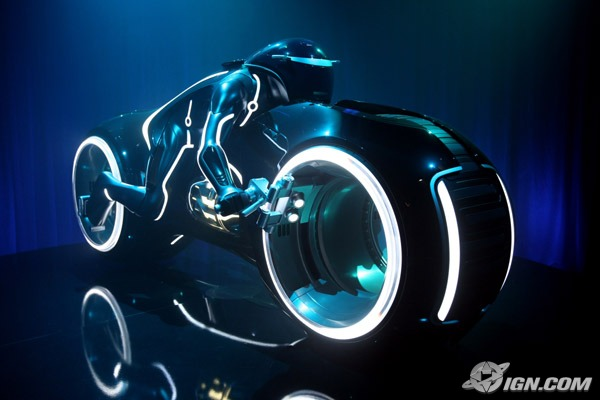
\includegraphics[width=\textwidth]{roz1/img/tron.jpg}\\\textit{a) Tron Legacy}
\end{minipage}
\begin{minipage}[b]{4cm}
\centering
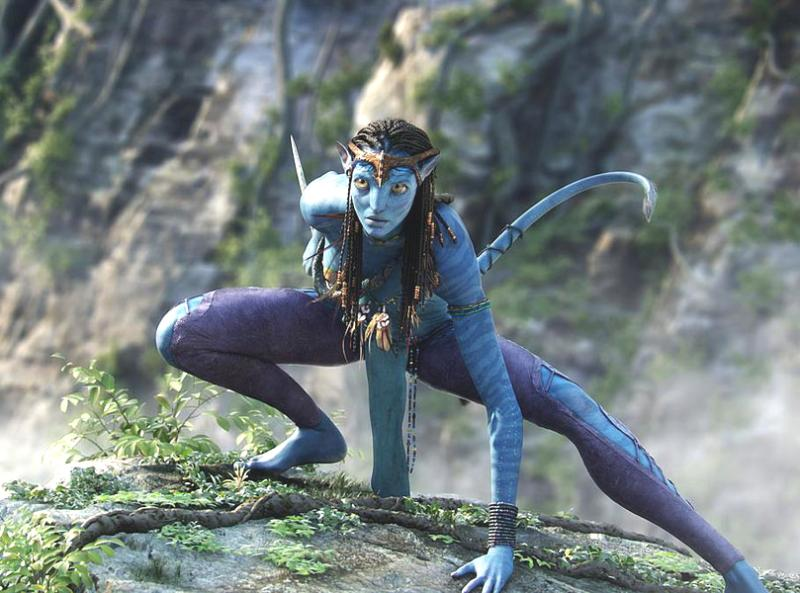
\includegraphics[width=\textwidth]{roz1/img/avatar.jpg}\\\textit{b) Avatar}
\end{minipage}
\begin{minipage}[b]{4cm}
\centering

\includegraphics[width=\textwidth]{roz1/img/shreck.jpg}\\\textit{c) Shrek}
\end{minipage}
\caption{Uj�cia filmowe stworzone za pomoc� technik komputerowych}
\label{fig:filmy_rt}
\end{center}
\end{figure}


\section{Motywacja}
\label{sec:chapter1:Motywacja}
G��wnym bod�cem motywacyjnym do napisania tej pracy by�a ch�� poszerzenia dotychczasowej wiedzy na temat  przy�pieszania oblicze� przy pomocy nowej technologii NVIDIA CUDA. Dodatkowymi czynnikami motywacyjnymi by�o zami�owanie do grafiki komputerowej oraz do tworzenia aplikacji oblicze� czasu rzeczywistego. Na co dzie� zajmuj� si� programowaniem gier/aplikacji na komputery klasy PC oraz urz�dzenia mobilne. Uwa�am, �e w przysz�o�ci przedstawiona przeze mnie w tej pracy metoda �ledzenia promieni b�dzie mia�a zastosowanie w grach oraz aplikacjach wykorzystuj�cych grafik� czasu rzeczywistego.


\section{Terminologia wykorzystywana w pracy}
\label{sec:chapter1:terminologia}
\begin{itemize} 
\item Developer - Tw�rca/programista aplikacji
\item CUDA - Technologia stworzona przez firm� NVIDIA w 2007 roku. Umo�liwia r�wnoleg�e obliczenia na mikroprocesorach karty graficznej
\item Raytracing - metoda generowania obrazu za pomoc� �ledzenia promieni.
\item Benchmark - Aplikacji testowa, kt�ra profiluje wydajno�� i zbiera informacje.
\item Warp - blok w�tk�w przydzielony na multiprocesor
\item DirectX - technologia graficzna firmy Microsoft. Umo�liwia wy�wietlanie wysokiej jako�ci grafiki 2D/3D.
\item Aliasing - Zdeformowany, o z�ej jako�ci obraz kt�ry powstaje podczas rastaryzacji, powodowany przez zbyt ma�a cz�stotliwo�� pr�bkowania na pojedy�czy pixel obrazu. Przeciwdzia�a si� temu efektowi poprzez antyaliasing oraz w raytracingu poprzez super-sampling
\item Super-sampling - spos�b na zwi�kszenie jako�ci generowanych scen. Polega na �ledzeniu wielu promieni �wietlnych na pojedy�czy pixel generowanego obrazu.
\end{itemize} 


\section{Dost�pne technologie, pozwalaj�ce zr�wnolegli� obliczenia na kartach graficznych}
\label{sec:chapter1:Dost�pneTechnologie}
Poni�ej zaprez�towane zosta�y trzy wybrane technologi� wspomagaj�ce r�wnoleg�e  obliczenia na kartach graficznych. Niemniej jednak badania przeprowadzone i opisane w dalszej cz�ci pracy b�d� skupia�y si� na wykorzystaniu jednej z tych metod, a mianowicie technologii NVIDIA CUDA.


\subsection{Open Computing Language (OpenCL)}
Technologia tak zainicjowana zosta�a przez firm� Apple. Do inicjatywy i rozwijania tej technologii w��czy�y si� w p�niejszym czasie inne firmy takie jak: AMD, IBM, Intel, NVIDIA. W roku 2008 sformowana zosta�a grupa Khronos skupiaj�ca powy�sze firmy oraz wiele innych nale��cych do bran�y IT. Grupa ta czuwa nad rozwojem technologii OpenCL. 
Technologia tak pozwala na pisanie kodu kt�ry jest przeno�ny mi�dzy wieloma platformami: komputery, urz�dzenia przeno�ne, klastry obliczeniowe. OpenCL pozwala rozprasza� obliczenia na jednostki procesorowe CPU oraz na architektury graficzne GPU. Bardzo wa�n� zalet� OpenCL jest to, �e pisanie z u�yciem tej technologii nie jest zale�ne od sprz�tu na jakim b�dzie ona uruchamiana.

\subsection{ATI Stream Computing}
Technologia ta zosta�a stworzona przez firm� AMD. Za pomoc� tej platformy jeste�my w stanie przeprowadza� z�o�one obliczenia na sprz�cie produkowanym przez AMD.
W sk��d ca�ego pakietu ATI Stream Computing wchodzi autorski j�zyk ATI Brook+ i kompilator tego� j�zyka. Dodatkowo ATI wspiera developer�w w�asn� biblioteka matematyczna (AMD Core Math Library) oraz narz�dziami do profilowania wydajno�ci kodu (Strem Kernel Analyzer). Technologia ATI konkuruje od dawna z technologi� NVIDIA CUDA.


\subsection{NVIDIA CUDA}
CUDA (Compute Unified Device Architecture) jest technologia opracowan� przez firm� NVIDIA. Swoje pocz�tki CUDA mia�a w 2007 roku i do dzi� jest wiod�c� technologi� strumieniowego przetwarzania danych z wykorzystaniem uk�ad�w graficznych GPU. Dalszemu opisu niniejszej technologii po�wi�cony zostanie osobny rozdzia�.

\begin{figure}[h]
\begin{center}
\begin{minipage}[b]{4cm}
\centering

\includegraphics[width=\textwidth]{roz1/img/cuda_logo.jpg}\\\textit{a) Logo NVIDIA CUDA}
\end{minipage}
\begin{minipage}[b]{4cm}
\centering

\includegraphics[width=\textwidth]{roz1/img/ati_logo.jpg}\\\textit{b) Logo ATI Stream Computing}
\end{minipage}
\caption{Loga dw�ch konkurencyjnych ze sob� technologii przetwarzania r�wnoleg�ego na kartach graficznych}
\label{fig:cuda_ati}
\end{center}
\end{figure}


\clearpage

% ********** Rozdzia� 2 **********
\chapter{Cele pracy}
\label{sec:chapter2}


\section{Opracowanie techniki zr�wnoleglenia i przyspieszenia metody �ledzenia promieni przy u�yciu NVIDIA CUDA}
Celem niniejszej pracy jest przeniesienie a zarazem zr�wnoleglenie algorytmu �ledzenia promieni na procesory graficzne (GPU) firmy NVIDIA. Celem tak�e jest przy�pieszenie oblicze� standardowego wstecznego Raytracingu w celu jak najszybszego generowania obraz�w scen 3D.


\section{Projekt uniwersalnej aplikacji - benchmark}
W ramach projektu napisany zosta� uniwersalny system Raytracingu dzia�aj�cy na wielo rdzeniowych procesorach komputerowych (CPU), a tak�e na kartach graficznych (GPU) firmy NVIDIA kt�re obs�uguj� technologie NVIDIA CUDA. Aplikacja testowa jest benchmarkiem, kt�ry jest w stanie przetestowa� zadane sceny 3D na wielu r�nych konfiguracjach sprz�towych. Aplikacja ma za zadanie po uruchomieniu na komputerze u�ytkownika, testowa� wszelkie sceny z odpowiedniego katalogu. Dodatkowo zbiera� potrzebne informacje o sprz�cie u�ytkownika oraz czasy generowania obraz�w z ka�dej ze scen. Po przeprowadzeniu wszelkich test�w aplikacja jest w stanie wysla� na adres e-mail developera (w tym przypadku autora pracy) wszelkie zgromadzone dane.

% ********** Rozdzia� 3 **********
\chapter{Wprowadzenie do Raytracingu}
\label{sec:chapter3}


\section{Wst�pny opis}
\label{sec:chapter3:Wstep}
W rzeczywistym �wiecie promienie �wietlne rozchodz� si� od �r�d�a �wiat�a do obiekt�w znajduj�cych si� w �wiecie. Ka�de �r�d�o �wiat�a wysy�a niesko�czon� liczb� swoich promieni �wietlnych. Nast�pnie te promienie odbijaj�c si� od obiekt�w i trafiaj� do oczu obserwatora powoduj�c �e widzi on okre�lony kolor danego obiektu. Gdyby zaadaptowa� t� metod� do generowania realistycznej grafiki komputerowej, otrzymaliby�my niesko�czenie dok�adny i realistyczny obraz. 
Z racji jednak na to, �e sprz�t komputerowy ma ograniczone mo�liwo�ci, a metoda ta jest bardzo nie efektywn� metod� pod wzgl�dem obliczeniowym. Najszerzej stosowan� metod� �ledzenia promieni jest wsteczne �ledzenie promieni (backward raytracing). W odr�nieniu od post�powego algorytmu �ledzenia promieni (forward raytrcing), kt�re opiera si� na generowaniu jak najwi�kszej liczby promieni dla ka�dego �r�d�a �wiat�a. Algorytm wstecznego �ledzenia promieni zak�ada, �e promienie �ledzone s� od obserwatora, poprzez scen� do obiekt�w z kt�rymi koliduj�. Poni�ej przedstawiony jest pogl�dowy rysunek �ledzenia pojedynczego promienia od obserwatora poprzez okre�lony pixel na ekranie: \ref{fig:barwa_pixela}

\begin{figure}[h]
	\centering
		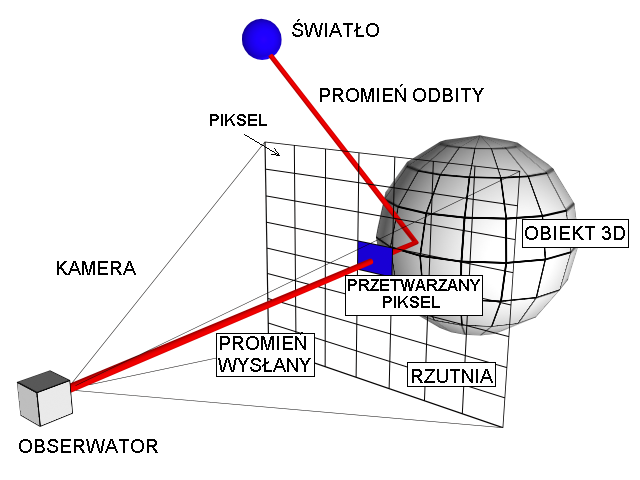
\includegraphics[width=\textwidth]{roz3/img/barwa_pixela.png}
	\caption{Spos�b okre�lania barwy piksela w raytracigu}
	\label{fig:barwa_pixela}
\end{figure}


\begin{figure}[h]
	\centering
		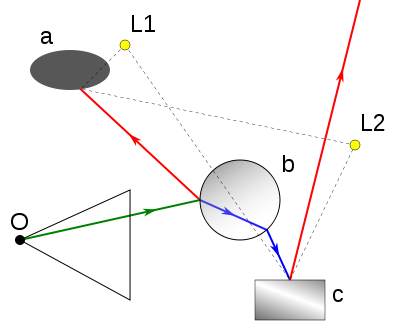
\includegraphics[width=\textwidth]{roz3/img/rekursywny_algorytm.png}
	\caption{Zasada dzia�ania rekursywnego algorytmu ray tracingu}
	\label{fig:rekursywny_algorytm}
\end{figure}


\section{Rekursywna metoda �ledzenia promieni}
\label{sec:chapter3:RekursywnaMetoda}
Przy omawianiu wstecznej metody �ledzenia promieni warto wspomnie� o raytracingu rekursywnym. W zagadnieniu tym bada si� rekurencyjnie promienie odbite zwierciadlane oraz za�amane, kt�re powsta�y z kolizji promieni pierwotnych 
z obiektami na scenie. Tak wi�c �ywotno�� promienia pierwotnego wcale nie ko�czy si� w momencie kolizji z obiektem sceny. To czy z danego promienia pierwotnego wygenerowane zostan� kolejne promienie w bardzo du�ej mierze zale�y od materia�u jakim pokryty jest dany obiekt sceny. Z pomoc� tego rekursywnej metody �ledzenia promieni jeste�my w stanie zasymulowa� obiekty lustrzane oraz obiekty p�przezroczyste. Rekurencja w tej metodzie trwa do osi�gni�cia maksymalnego stopnia zag��bienia. Kolor wynikowy danego pojedynczego Pixela powstaje z sumy kolor�w, obiektu w jaki trafi� promie� pierwotny oraz kolor�w obiekt�w w jakie trafi�y promienie pierwotne. Poni�ej przedstawiony jest pogl�dowy schemat zasady dzia�ania rekursywnej metody �ledzenia promieni: \ref{fig:rekursywny_algorytm}


\section{Przedstawienie algorytmu �ledzenia promieni}
\label{sec:chapter3:PrzedstawienieAlgorytmu}
�ledzenie promieni przez scen� rozpoczyna si� od obserwatora okre�lanego cz�sto jako kamery wyst�puj�cej na scenie. Przez ka�dy pixel ekranu �ledzone s� promienie kt�re poruszaj� si� po scenie. Gdy kt�ry� ze �ledzonych promieni napotka obiekt i zacznie z nim kolidowa�. 





\section{Przyk�ad sz�sty}

Oto przyk�adowy wydruk:
\begin{lstlisting}[language=C,style=outcode]
/* ta funkcja oblicza a+b */
int sum(int a, int b) 
{
	int suma=0;

	suma=a+b;

	return suma;
}
\end{lstlisting}










%% ********** Podzi�kowania **********
\clearpage
\chapter*{Podzi�kowania}
Chcia�bym bardzo podzi�kowa� mojemu promotorowi za opiek� naukow� oraz cenne rady podczas pisania tej pracy.\\

Dodatkowo bardzo dzi�kuj� moim rodzicom oraz mojej dziewczynie. Bez ich wsparcia i bod�c�w motywacyjnych powstanie tej pracy nie by�o by mo�liwe.\\

Na ko�cu lecz nie mniej wa�ne podziekowania dla mojego sprz�tu, kt�ry du�o wycierpia� podczas powstawania niniejszej pracy. Karta graficzna wymieniana byla trzy razy...
 

% ********** Koniec podzi�kowa� **********

%% *************** Spis symboli i skr�t�w ***************

% ******************************************************************************
% W tym miejscu mo�esz stworzy� w�asn� list� symboli i skr�t�w.
% Wystarczy jedynie oznaczy� miejsce pierwszego wyst�pienia symbolu etykiet�
% aby na li�cie symboli otrzyma� numer strony, na kt�rej on wyst�puje.
% ******************************************************************************

\chapter*{Spis symboli i skr�t�w}

\begin{center}
\small
\begin{longtable}{lp{3.0in}c}
\toprule
\multicolumn{1}{c}{Skr�t}
                & \multicolumn{1}{c}{Opis}
                                & \multicolumn{1}{c}{Definicja}\\ \midrule\addlinespace[2pt] \endhead
\bottomrule\endfoot
GAE                             & Google App Engine
                                & \pref{sym:GAE}\\
JSON                             & JavaScript Object Notation
                                & \pref{sym:JSON}\\
HTTP                            & Hypertext Transfer Protocol
                                & \pref{sym:HTTP}\\
OAuth                            & Open Authorization
                                & \pref{sym:OAuth}\\
                                
\end{longtable}
\end{center}

% *************** Koniec spisu symboli i skr�t�w ***************

%% ********** Rozdzia� 1 **********
\chapter{Wst�p}
\label{sec:chapter1}


\section{Wprowadzenie}
\label{sec:chapter1:Wprowadzenie}
Autostop od lat jest jedn� z najciekawszych metod podr�owania. Dla jednych jest form� taniego przebycia drogi z punktu A do B, dla innych sposobem na �ycie. 

Podr�e autostopem pomimo niezliczonej ilo�ci zalet: niskiego kosztu, mo�liwo�� prze�ycia przygody oraz spotkania interesuj�cych ludzi maj� dwie fundamentalne wady: nie mamy gwarancji, �e uda nam si� przeby� dany odcinek drogi w okre�lonym czasie, a osoba, z kt�r� b�dziemy podr�owa�, nie oka�e si� szale�cem, kt�ry zagrozi naszemu bezpiecze�stwu.

W mojej pracy stara�em si� stworzy� rozwi�zanie, kt�re pozwoli w znacz�cy spos�b usprawni� podr�e autostopem, zapewni� ich bezpiecze�stwo i wyeliminowa� wady tradycyjnego rozwi�zania, zachowuj�c przy tym wszystkie jego zalety. 

mobiStopowicz jest zgodny z najnowszymi trendami internetowymi, technologicznymi oraz spo�ecznymi. Jest zintegrowanany z najwi�kszym i najpr�niej rozwijaj�cym si� portalem spo�eczno�ciowym, wykorzystuje najnowsze rozwi�zania serwerowe, nastawiony jest na u�ytkownik�w b�d�cych w ruchu. Promuje racjonaln� i oszcz�dn� gospodark� zasobami.

Nazwa systemu pochodzi od dw�ch s��w: mobilny i autostopowicz. Mobilny, bo przeznaczony dla telefon�w kom�rkowych (mobile phones), autostopowicz, bo jest to system przeznaczony dla nowoczesnych autostopowicz�w.

\section{Motywacja}
Motywacja do zaj�cia si� przeze mnie tematem mia�a 3 g��wne �r�d�a:
\begin{itemize}
    \item Zami�owanie do system�w mobilnych oraz ich efektywnego wykorzystania w czynieniu �ycia �atwiejszym.
	\item Zainteresowanie autostopem jako sposobem podr�owania po��czone z kilkoma niemi�ymi do�wiadczeniami zwi�zanymi z t� form� podr�y.
	\item Niech�� do wielkiego marnotrawstwa jakim s� bardzo popularne na polskich i zagranicznych drogach "jednoosobowe samochody", tzn. takie, w kt�rych podr�uje jedynie kierowca. 
\end{itemize}

Po pojawieniu si� pomys�u na prac�, skonsultowa�em si� ze znajomymi, specjalistami z bran�y oraz promotorem. Przejrza�em dost�pne rozwi�zania i doszed�em do wniosku, �e po��czenie autostopu z telefonem kom�rkowym mo�e stworzy� �wietny system dla podr�uj�cych.

\section{Cel pracy}
Celem pracy jest stworzenie mobilnego systemu na platform� BlackBerry wspieraj�cego podr�e autostopem. Powsta�y system ma na celu wyeliminowanie niedoskona�o�ci zwyk�ych podr�y autostopem, zachowuj�c wszystkie zalety tradycyjnej metody. Powsta�y system pozwala na:
\begin{itemize}
    \item Jasne okre�lenie sk�d, dok�d i kiedy chcemy dojecha�.
    \item Zweryfikowanie to�samo�ci zar�wno kierowcy jak i pasa�era.
    \item Sparowanie pasa�era oraz kierowcy zar�wno z du�ym wyprzedzeniem jak i Ad hoc w czasie rzeczywistym.
\end{itemize}

ponadto:
\begin{itemize}
	\item System jest skalowalny i globalny, b�dzie w stanie obs�u�y� du�e ilo�ci u�ytkownik�w na ca�ym �wiecie
  \item System jest �atwo rozszerzalny o nowe platformy klienckie (Android, iPhone, etc.)
  \item Algorytm wykorzystany do parowania u�ytkownik�w serwis�w jest prosty, skalowalny i efektywny.
\end{itemize}

\section{Terminologia wykorzystywana w pracy}
\begin{itemize}
	\item podr� - przemieszczenie si� z punktu A do punktu B rozpoczynaj�ce si� w okre�lonym momencie czasowym T
	\item aplikacja kliencka - aplikacja dost�powa do systemu mobiStopowicz instalowana na urz�dzeniu typu BlackBerry
	\item aplikacja serwerowa - aplikacja znajduj�ca si� po stronie serwera obs�uguj�ca ��dania wysy�ane przez aplikacj� klienck�
	\item u�ytkownik systemu - osoba zarejestrowana w systemie mobiStopowicz, posiadaj�ca zainstalowan� na swoim urz�dzeniu mobilnym aplikacj� klienck�
	\item kierowca - u�ytkownik systemu, kt�ry posiada samoch�d i poszukuje os�b do wsp�lnej podr�y
	\item oferta podr�y - oferta kierowcy zamieszczona w systemie. Zawiera informacje o tym sk�d, dok�d i kiedy podr�uje kierowca. Mo�e zawiera� dodatkowe preferencje co do potencjalnych pasa�er�w.
	\item pasa�er - u�ytkownik systemu poszukuj�cy odpowiadaj�cych mu ofert podr�y
	\item ��danie podr�y - poszukiwanie oferty podr�y o zadanych parametrach przez pasa�era
	\item sparowanie - proces w wyniku kt�rego kierowca oraz pasa�er zostan� ze sob� skontaktowani, poniewa� oferta podr�y kierowcy i ��danie podr�y pasa�era pokrywaj� si�.
	
\end{itemize}

\section{Za�o�enia}
\begin{enumerate}
		\item System sk�ada si� z dw�ch cz�ci: aplikacji po stronie serwera opartej o platform� Google App Engine w wersji 1.3 oraz aplikacji klienckiej przeznaczonej na platform� BlackBerry w wersji 5.0 i wy�szej.
    \item Praca in�ynierska jest opisem powsta�ego rozwi�zania, a tak�e drogi, jak� musia�em pokona� od pomys�u do produktu.
\end{enumerate}

\section{Dzia�anie systemu w praktyce}
Oto przyk�ady sytuacji w jakich system mo�e sprawdzi� si� w prawdziwym �yciu.
\subsection{Z punktu widzenia kierowcy}
Mariusz jest trzydziestoletnim architektem. Mieszka i pracuje w Warszawie. Jego pasj�, opr�cz sztuk walki, jest windsurfing. Dzi�, tzn. w pi�tek, wychodzi wcze�niej z pracy, gdy� wybiera si� na ca�y weekend na Hel pop�ywa� na windsurfingu. Nie martwi si�, i� b�dzie jecha� ca�� drog� sam swoim 5-cio osobowym samochodem. W �rod� wys�a� ofert� do systemu mobiStopowicz i jeszcze tego samego dnia do jego podr�y do��czyli Dominik i Micha�, r�wnie� zapaleni windsurferzy. Mariusz dowiedzia� si� tego, przegl�daj�c ich profile i zdj�cia na Facebook'u. W czwartek rano do podr�y do��czy�a Kasia, kt�ra jedzie odwiedzi� rodzic�w i  poimprezowa� nad morzem. \\
\newline
15.00: Mariusz w�a�nie wychodzi z biura. Jest ju� spakowany, deska na dachu jego auta b�yszczy w popo�udniowym s�o�cu. \\
15.15: Mariusz odbiera Dominika i Micha�a z Centrum, ruszaj� w kierunku Ochoty odebra� Kasi�. \\
15.30: Kasia w�a�nie wygodnie zasiad�a na tylnej kanapie. "-No to kierunek Hel" m�wi Mariusz i ruszaj� w drog�. \\

Jeszcze podczas jazdy Dominik i Micha� dogaduj� si� z Mariuszem, �e b�d� wraca� razem w niedziel� wieczorem. Po dotarciu na miejsce ka�dy rusza w kierunku swojego pensjonatu. Spotkaj� si� wieczorem, gdy� Kasia zaprosi�a ich na wsp�ln� imprez�[...]

\subsection{Z punktu widzenia pasa�era}
Klaudia jest studentk� drugiego roku medycyny w Warszawie. Mia�a dzisiaj wraca� do swojego rodzinnego miasta Gr�jca, pom�c rodzicom przy zbieraniu jab�ek w sadzie, gdy� sezon w pe�ni. Niestety, w�a�nie uciek� jej ostatni PKS. Ju� mia�a dzwoni� do domu, by kto� po ni� przyjecha�, gdy przypomnia�a sobie o systemie, o kt�rym m�wi�a jej kole�anka, taki nowoczesny autostopowicz. Jeden SMS i ju� zna�a nazw� : "mobiStopowicz". Szybko �ci�gn�a aplikacj� na sw�j telefon, nie musia�a si� nawet rejestrowa�, gdy� do systemu mog�a zalogowa� si� za pomoc� swojego konta na Facebook'u. Wpisa�a: punkt startu podr�y - "Dworzec zachodni, Dworzec PKS", punkt zako�czenia - "Gr�jec", czas startu - "Teraz". Szukaj, 3 oferty odnalezione, najbli�sza za 15 minut. "Ale czy to aby bezpieczne, przecie� kierowca mo�e okaza� si� jakim� szale�cem?" - pomy�la�a. Sprawdzi�a profil i to rozwia�o jej wszelkie obawy. Okaza�o si�, �e kierowc� zamieszczaj�cym pierwsz� ofert�, jest Karol, brat kole�anki z klasy z podstaw�wki. Jeszcze jedno klikni�cie i ju� s� um�wieni. Za 5 min Karol podjedzie po ni� na dworzec. "Ciekawe czy Karol jest nadal taki przystojny"' pomy�la�a Klaudia [...]



% ********** Koniec rozdzia�u **********

%% ********** Rozdzia� 2 **********
\chapter{Rekonesans}
\label{sec:chapter2}
W tym punkcie zapozna�em si� z istniej�cym stanem wiedzy oraz istniej�cymi rozwi�zaniami, zrobi�em kalkulacje ilu potencjalnie u�ytkownik�w mo�e mie� system oraz podj��em decyzj�, o tym, i� rzeczywi�cie potrzebny jest kolejny system dla autostopowicz�w, pomimo istnienia pozornie podobnych rozwi�za�.

\section{Przegl�d literatury}
Literatury traktuj�cej o nowoczesnych formach autostopu jest niezwykle ma�o. Jedyn� prac�, jak� uda�o mi si� znale�� na ten temat to opracowanie stworzone przez Research Center firmy Nokia \cite{EmptySeats}. W dokumencie starano si� dokona� szacunk�w rozmiaru rynku dla tej formy podr�owania, przedstawiono projekt systemu na wysokim poziomie abstrakcji, a tak�e zaproponowano model rozliczania u�ytkownik�w. W dokumencie autorzy niezwykle entuzjastycznie podchodz� do tematu i widz� w nim wielki potencja�. 

\section{Istniej�ce rozwi�zania}
Na rynku istnieje wiele rozwi�za� maj�cych na celu pomoc autostopowiczom w ich podr�ach. Poczynaj�c od najprostszych system�w typu tablica og�osze�, przez proste aplikacje internetowe po z�o�one systemy o bogatej liczbie funkcji. W tym punkcie przyjrz� si� rozwi�zaniom zar�wno przeznaczonym na rynek krajowy jak i o globalnym zasi�gu.
\subsection{Systemy polskie}
\begin{itemize}
    \item www.autostop.com.pl \\
Prosty polski system webowy s�u��cy do umawiania si� do wsp�lnych podr�y. Umo�liwia proste dodawanie ofert kierowc�w oraz proste wyszukiwanie dost�pnych ofert.
    \item www.autostopem.net \\
Serwis o podr�owania autostopem udost�pniaj�cy r�wnie� forum pozwalaj�ce znale�� kompana do wsp�lnej podr�y. Brak zaawansowanych mechanizm�w wyszukiwania.
    \item www.nastopa.pl \\
Troch� bardziej rozbudowany serwis, kt�ry poza podstawowymi funkcjami udost�pnia kilka dodatkowych opcji jak kalkulator koszt�w czy pomiar odleg�o�ci.

\end{itemize}


\subsection{Systemy globalne}
\begin{itemize}
    \item www.erideshare.com \\
Serwis o do�� du�ej popularno�ci za granic�. Udost�pnia podstawowe opcje wzbogacone o funkcje serwisu spo�eczno�ciowego.
    \item rideshareonline.com \\
Serwis sk�adaj�cy si� z kilku us�ug, mi�dzy innymi us�ugi dla autostopowicz�w. Posiada bardzo du�� ilo�ci funkcji, elementy spo�eczno�ciowe oraz mo�liwo�� zbierania statystyk i historii u�ytkownika. Nie posiada jednak wersji mobilnej. 

\end{itemize}

\subsection{Podsumowanie}
�aden z polskich system�w nie mo�e zosta� okre�lony mianem rozwi�zania dojrza�ego i w pe�ni funkcjonalnego. Systemy te udost�pniaj� niemal�e ten sam, ubogi zestaw funkcji i nie mog� spe�ni� potrzeb nawet mniej wymagaj�cych u�ytkownik�w. Sytuacja po�r�d system�w obcoj�zycznych jest lepsza. Na szczeg�ln� uwag� zas�uguje "rideshareonline.com" dopracowany i funkcjonalny.

\begin{table}[h]
\centering
\begin{tabularx}{\textwidth}{| c | X | X | X | X | X |}

\hline
Serwis & Weryf. to�samo�ci & Funkcje spo�eczno�ciowe & Wersja mobilna & Zaaw. wyszukiwanie & Preferen. \\
\hline
autostop.com.pl & - & - & - & - & - \\ \hline
autostopem.net & - & - & - & - & - \\ \hline
nastopa.pl & - & - & - & - & - \\ \hline
erideshare.com & \checkmark & \checkmark & - & \checkmark & - \\ \hline
rideshareonline.com  & \checkmark & \checkmark & - & \checkmark & \checkmark \\ \hline


\end{tabularx}
\caption{Por�wnanie istniej�cych na rynku system�w dla autostopowicz�w}
\label{tab: zestawienie}
\end{table}

\section[Innowacyjno�� rozwi�zania]{Innowacyjno�� rozwi�zania, czyli czy rzeczywi�cie potrzebny jest kolejny system?}

Jak opisa�em w poprzednim punkcie istnieje na rynku wiele system�w, kt�re w mniejszym lub wi�kszym stopniu maj� wspiera� parowanie kierowc�w i pasa�er�w do wsp�lnej podr�y. Czy warto wi�c tworzy� kolejny system? Moim zdaniem tak. Moje rozwi�zanie posiada 3 cechy kt�re czyni� je innowacyjnym:
\begin{enumerate}
    \item Aplikacja przeznaczona jest na urz�dzenia mobilne. W zwi�zku ze specyfik� urz�dzenia mobilnego us�uga dost�pna jest w ka�dym miejscu, o ka�dej porze.
    \item Aplikacja nie wymaga tworzenia nowego konta, do uwierzytelniania wykorzystywane jest konto Facebook'owe.
    \item Osoby w systemie nie s� anonimowe. To�samo�� osoby jest potwierdzana przez publiczne konto Facebook'owe oraz znajomych u�ytkownika, czyli kontekst w kt�rym dany profil wyst�puje. Jest to nowatorskie podej�cie do zapewnienia bezpiecze�stwa.
\end{enumerate}

\section{Potencjalne grono odbiorc�w}
Potencjalnym u�ytkownikiem us�ugi jest ka�dy podr�ny, wi�c w rzeczywisto�ci przynajmniej po�owa populacji. Szacuje si�, �e na �wiecie obecnie znajduje si� oko�o 600mln aut \cite{WikiCars}. Ka�de z nich mo�e by� u�ywane do wsp�lnego podr�owania wspieranego przez system mobiStopowicz. Potencjalny rynek jest wi�c olbrzymi. Zgodnie z tabel� \ref{tab: iloscSamochodowNaMieszkanca} widzimy, �e w krajach rozwini�tych przynajmniej, co druga osoba ma samoch�d. Mo�emy na tej podstawie wysnu� tez�, i� spora cz�� samochod�w jest wykorzystywane jedynie przez kierowc�w(bo prawie ka�dy ma swoje auto). W krajach tych system mobiStopowicz ma du�y potencja�, w szczeg�lno�ci przy rosn�cych cenach benzyny i ekologicznych nastroj�w spo�ecznych.
\begin{table}
\centering
\begin{tabular}{|l|l|l|}
\hline
Lp. & Pa�stwo & Samochody na 1000 mieszk. \\ 
\hline
1 & USA & 765 \\ 
\hline
2 & Luksemburg & 686 \\ 
\hline
3 & Malezja & 641 \\ 
\hline
4 & Australia & 619 \\ 
\hline
5 & Malta & 607 \\ 
\hline
6 & W�ochy & 566 \\ 
\hline
7 & Kanada & 563 \\ 
\hline
8 & Nowa Zelandia & 560 \\ 
\hline
9 & Austria & 558 \\ 
\hline
10 & Niemcy & 546 \\ 
\hline
\end{tabular}
\caption{Pa�stwa o najwi�kszej ilo�ci aut w przeliczeniu na mieszka�ca, �r�d�o: \cite{WikiCars} }
\label{tab: iloscSamochodowNaMieszkanca}
\end{table}




% ********** Koniec rozdzia�u **********

% \chapter{Algorytm parowania kierowc�w i pasa�er�w do wsp�lnej podr�y}
\label{sec:chapter3}
Wykorzystany przeze mnie algorytm jest niezwykle prosty, a zarazem wyj�tkowo skuteczny i skalowalny.

\section{Za�o�enia}

\begin{itemize}
    \item Podr� jest to przemieszczenie si� z punktu A do punktu B, kt�re rozpoczyna si� w momencie czasowym T.
    \item Algorytm uwzgl�dnia preferencje, tzn. parametry, kt�re musz� si� zgadza� dla ka�dej ze stron (kierowcy i pasa�era) bior�cych udzia� w podr�y.
\end{itemize}

\section{Dzia�anie algorytmu}
Algorytm mo�e zosta� uruchomiony w dw�ch trybach: poszukiwania oferty kierowcy spe�niaj�cej wymagania pasa�era oraz w trybie poszukiwania ��dania pasa�era spe�niaj�cego wymagania kierowcy.  W aplikacji mobiStopowicz wykorzystywany jest jedynie pierwszy tryb. Po uruchomieniu algorytmu baza danych przeszukiwana jest w poszukiwaniu oferty spe�niaj�cej zadane kryteria, tzn:
\begin{enumerate}
    \item zgodno�� pod wzgl�dem punktu startu
    \item zgodno�� pod wzgl�dem punktu ko�ca
    \item zgodno�� pod wzgl�dem czasu rozpocz�cia podr�y
\end{enumerate}
w drugiej kolejno�ci brane s� pod uwag� kryteria dodatkowe takie jak:
\begin{itemize}
    \item preferencje wiekowe co do kierowcy/pasa�era
    \item preferencja palenie zabronione/palenie dozwolone
\end{itemize}

Po odnalezieniu listy ofert spe�niaj�cej zadane warunki wynik zwracany jest do u�ytkownika. Schemat blokowy algorytmu zosta� przedstawiony na rysunku \ref{fig:schematBlokowyAlgorytmu}.

Algorytm jest rozszerzalny o nowe parametry. Istnieje na przyk�ad mo�liwo�� dodania nowych preferencji. W przypadku, gdybym zdecydowa� si� wprowadzi� funkcje rozliczalno�ci dla u�ytkownik�w mo�na doda� nowy parametr okre�laj�cy, czy kierowca oczekuje od pasa�era wynagrodzenia oraz jaka jest jego wysoko��.

\begin{figure}[h]
\centering.png.p[bb=0 0 976 ,
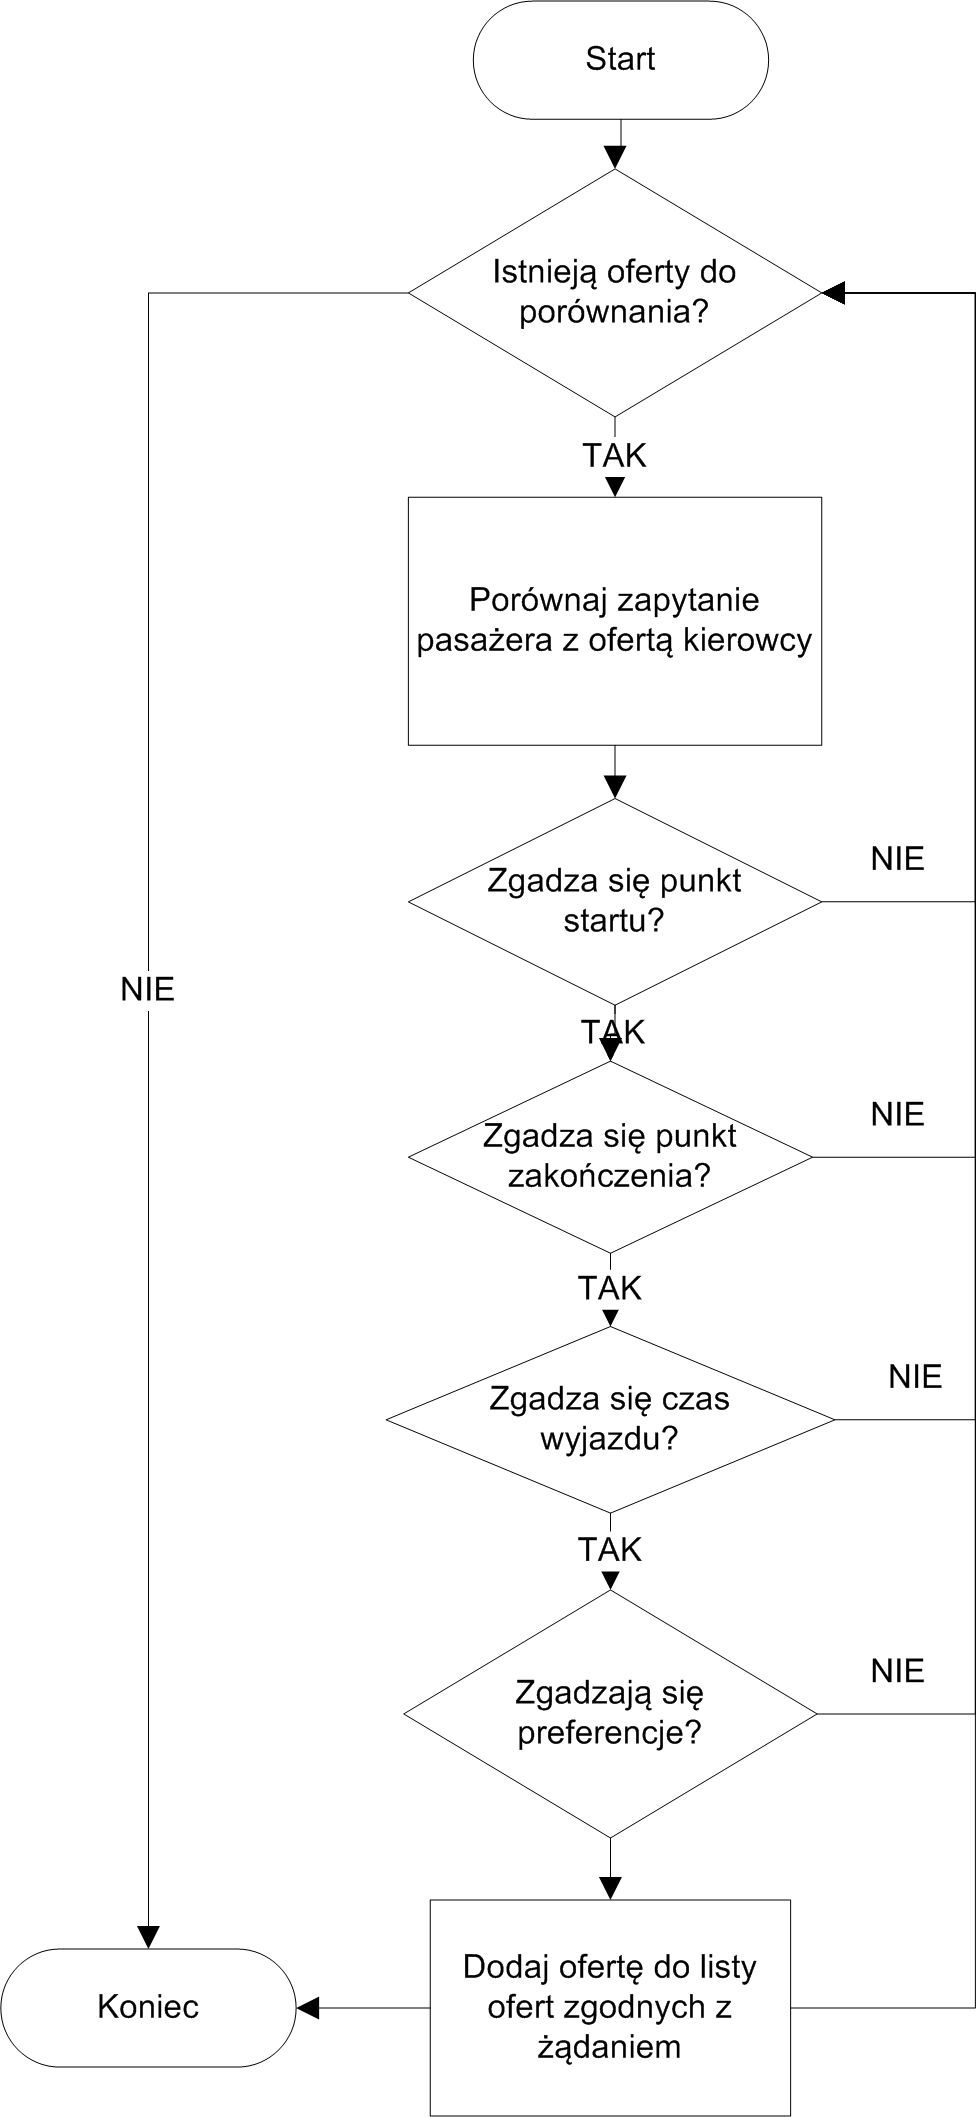
\includegraphics [height=500px]{chap3//algorytm}
\caption{Schemat blokowy dzia�ania algorytmu}
\label{fig:schematBlokowyAlgorytmu}
\end{figure}

\section{Z�o�ono�� czasowa algorytmu}
Algorytm ma z�o�ono�� rz�du O(N), jest to niezwykle istotne w skalowalnych systemach o du�ej ilo�ci u�ytkownik�w, a takim systemem jest w�a�nie mobiStopowicz.

% \chapter{Architektura}
\label{sec:chapter4}

\section{Serwisy, protoko�y, techniki i technologie wykorzystane w aplikacji}
Aplikacja ca�ymi gar�ciami czerpie z najnowszych rozwi�za� dost�pnych na rynku IT. Na wst�pie nale�y przybli�y� najwa�niejsze z nich.
\subsection{facebook.com}
Serwis spo�eczno�ciowy, kt�ry pozwala zarejestrowanym u�ytkownikom tworzy� sieci, grupy tematyczne, dzieli� si� wiadomo�ciami i grupami. Facebook pozwala r�wnie� na tworzenie aplikacji wykorzystuj�cych zasoby znajduj�ce si� w serwisie. mobiStopowicz jest jedn� z takich aplikacji.
\subsubsection{OAuth 2.0}
\label{sym:OAuth}
OAuth (Open Authorization) jest otwartym standardem pozwalaj�cym u�ytkownikom dzieli� si� ich prywatnymi zasobami (zdj�ciami, plikami, kontaktami) znajduj�cymi si� w jednym serwisie z innymi serwisami bez konieczno�ci udost�pniania danych dost�powych innemu serwisowi. W wersji 2.0 skupiono si� na uproszczeniu protoko�u.
\subsubsection{Graph API}
Graph API jest kluczow� us�ug� platformy Facebook.com. Pozwala aplikacjom klienckim odczytywa� oraz zapisywa� dane z i do platformy. Udost�pnia prosty i ujednolicony mechanizm dost�pu do zasob�w takich jak kontakty, zdj�cia, wydarzenia.
\subsection{Google App Engine}
\label{sym:GAE}
GAE (Google App Engine) jest to platforma przeznaczona do tworzenia i hostowania skalowalnych aplikacji webowych udost�pnione u�ytkownikom w 2008r. przez firm� Google. GAE pozwala na tworzenie aplikacji w j�zyku Java oraz Python. 
\subsubsection{Datastore}
Jest to us�uga sk�adowania danych dostarczana wraz z platform� Google App Engine. Nie jest to tradycyjna, relacyjna baza danych. Dane w Datastore przechowywane s� w postaci obiekt�w konkretnego typu posiadaj�cych konkretne w�a�ciwo�ci.
\subsection{HTTP}
\label{sym:HTTP}
Jeden z fundament�w Internetu. HTTP (Hypertext Transfer Protocol ) jest protoko�em do przesy�ania dokument�w w sieci WWW. Udost�pnia znormalizowany spos�b komunikowania si� komputer�w ze sob�. Okre�la form� ��da� klienta dotycz�cych danych oraz form� odpowiedzi serwera. Jest protoko�em bezstanowym.
\subsection{JSON}
\label{sym:JSON}
JSON (JavaScript Object Notation) jest to lekki, tekstowy format wymiany danych.

\section{Realizacja}
System dzia�a w oparciu o architektur� typu klient-serwer. Zapytania przesy�ane s� z u�yciem protoko�u HTTP, a tre�� zapytania jest obiektem typu JSON. Architektura zosta�a przedstawiona na schemacie \ref{fig:architektura}.

Podczas tworzenia systemu stan��em przed wyborem formatu przesy�anych danych. Od pocz�tku wiedzia�em, �e u�yj� jednego z protoko��w tekstowych (poniewa� jest �atwy do odczytania przez cz�owieka w fazie rozwoju aplikacji). Do wyboru mia�em 2 najpopularniejsze formaty: JSON i XML.

Wybra�em JSON z nast�puj�cych powod�w:
\begin{itemize}
	\item JSON jest formatem du�o "l�ejszym". Narzut przez niego generowany jest nawet o 75\% mniejszy ni� w przypadku XML'a. Jest to niezwykle istotne w przypadku us�ug przeznaczonych dla urz�dze� mobilnych, w kt�rych nadal p�aci si� za przesy�ane jednostki danych, a ��cza maj� du�o wi�ksze ograniczenia przepustowo�ci, ni� w systemach stacjonarnych.
	\item Na wykorzystywane przeze mnie platformy dost�pne s� �wietne biblioteki wspieraj�ce obs�ug� tego formatu.
	\item Facebook udost�pnia dane w swoim API jako dane w formacie JSON, unikn��em wi�c konieczno�ci ��czenia wielu format�w w jednym systemie. 
\end{itemize}

\begin{figure}[h]
	\centering
		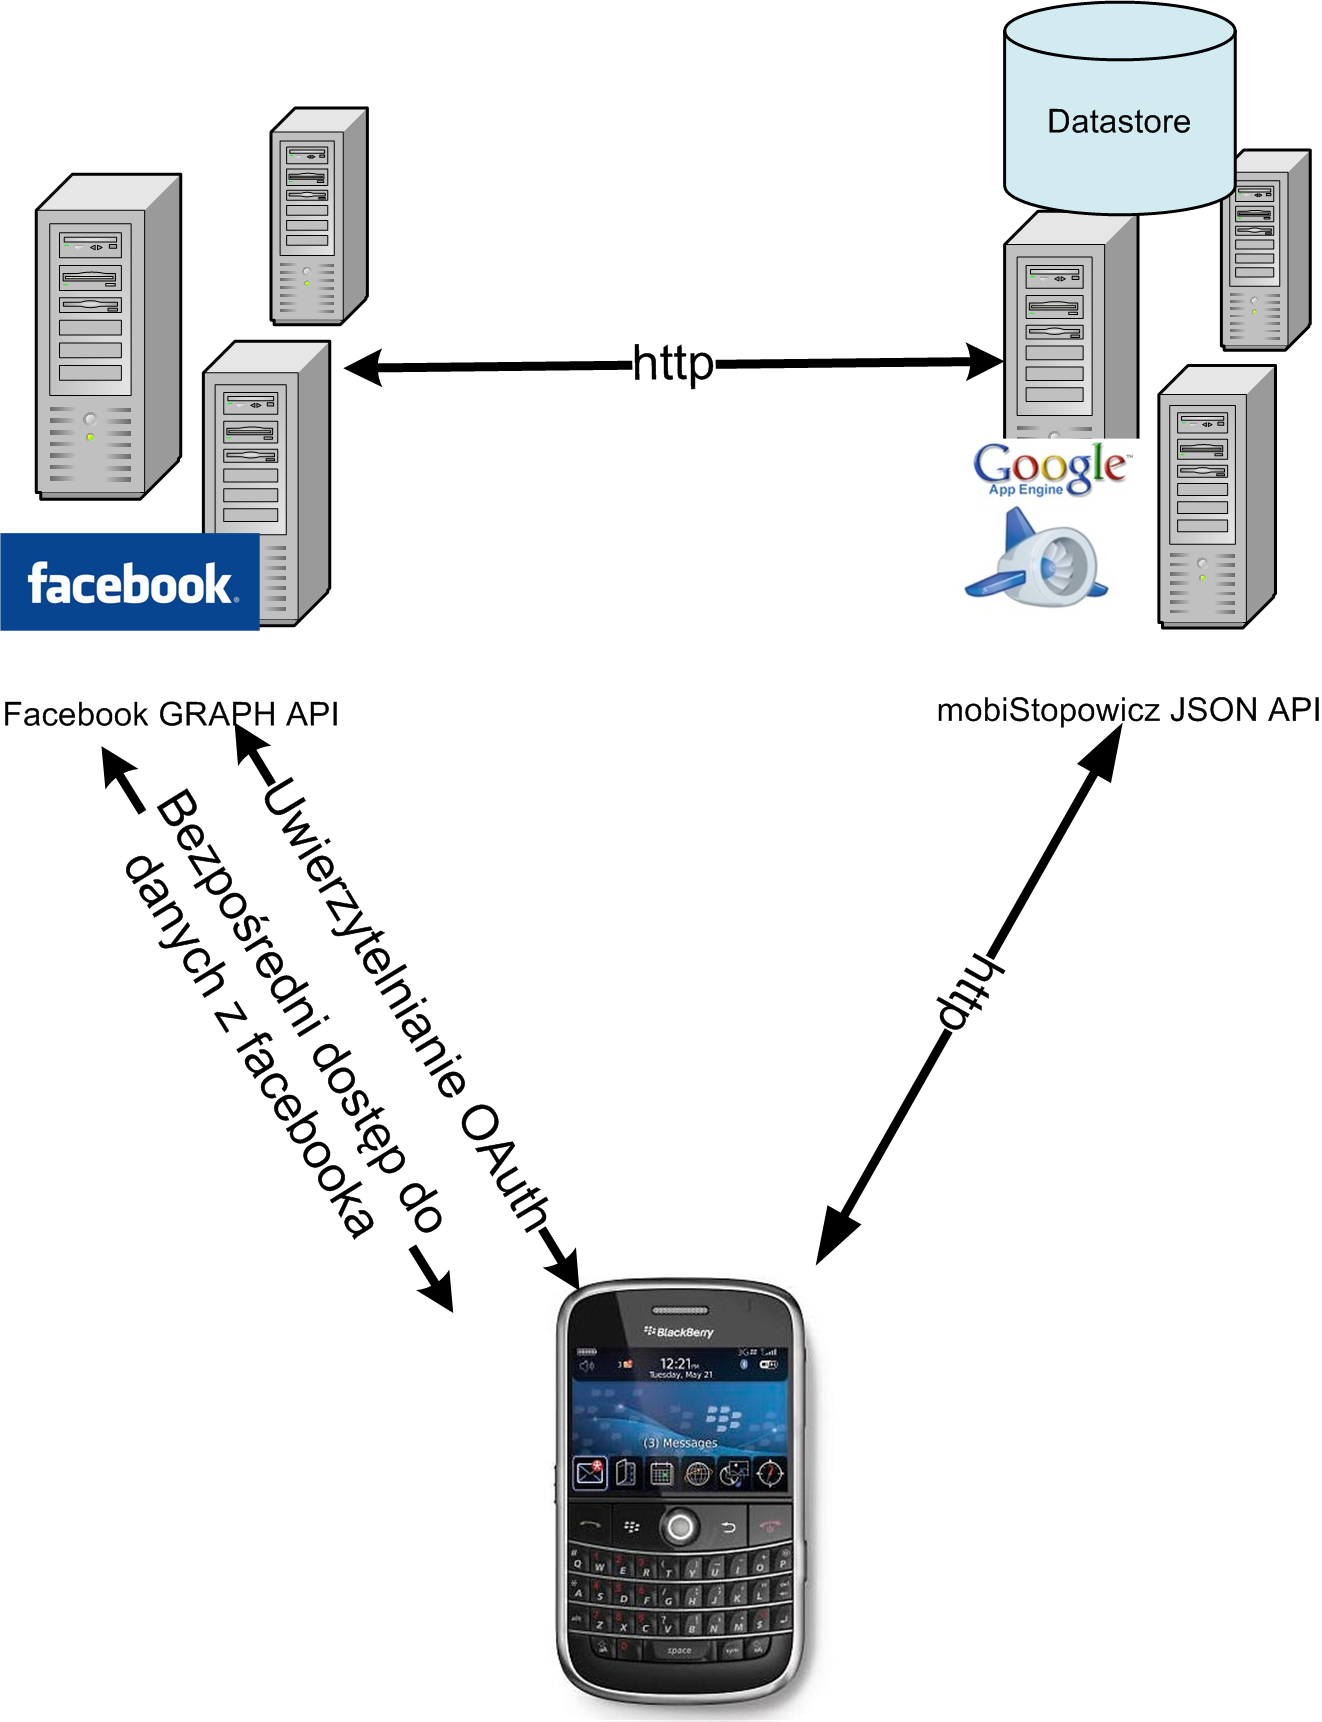
\includegraphics[width=\textwidth]{chap4/img/architektura}
	\caption{Architektura systemu}
	\label{fig:architektura}
\end{figure}

W systemie mo�emy wyr�ni� trzy g��wne komponenty:
\begin{enumerate}
	\item Aplikacja kliencka\\
	 S�u�y do komunikacji u�ytkownika z serwisem mobiStopowicz a tak�e z serwerem Facebook'a. Umo�liwia pe�n� interakcj� z us�ug�. 
	\item Aplikacja serwerowa\\
	Serce systemu. Jest odpowiedzialna za autoryzacj� i obs�ug� ��da� od u�ytkownik�w. Komunikuje si� r�wnie� z Facebook'iem.
	\item Serwis Facebook\\
	 Odpowiedzialny za uwierzytelnianie u�ytkownik�w. Pozwala tak�e na bezpo�redni dost�p do danych na nim zgromadzonych, np. do profili u�ytkownik�w.
\end{enumerate}
	


\subsection{Uwierzytelnianie}
Uwierzytelnianie przeprowadzane jest przy u�yciu protoko�u OAuth 2.0 i Facebook'a jako strony uwierzytelniaj�cej. W aplikacji mobiStopowicz otwierana jest wbudowana strona Facebook'a, kt�ra umo�liwia dokonanie logowania i udzielenia uprawnie� dost�pu do danych u�ytkownika dla aplikacji mobiStopowicz. Po poprawnym zalogowaniu, do aplikacji klienckiej zwracany jest token, kt�ry nast�pnie u�ywany jest do autoryzacji i identyfikowania u�ytkownika w komunikacji z serwerem. Od tej pory u�ytkownik jest identyfikowany w systemach mobiStopowicz oraz Facebook'u przy u�yciu tokenu dost�powego.
\subsection{Pierwsze po��czenie z serwerem mobiStopowicz}
Po uwierzytelnieniu u�ytkownika aplikacja kliencka posiada token dost�powy. Wys�anie dowolnego ��dania do serwera z do��czonym tokenem powoduje wywo�anie procedury zgodnie z rysunkiem \ref{fig:autentykacja}
\begin{figure}
	\centering
		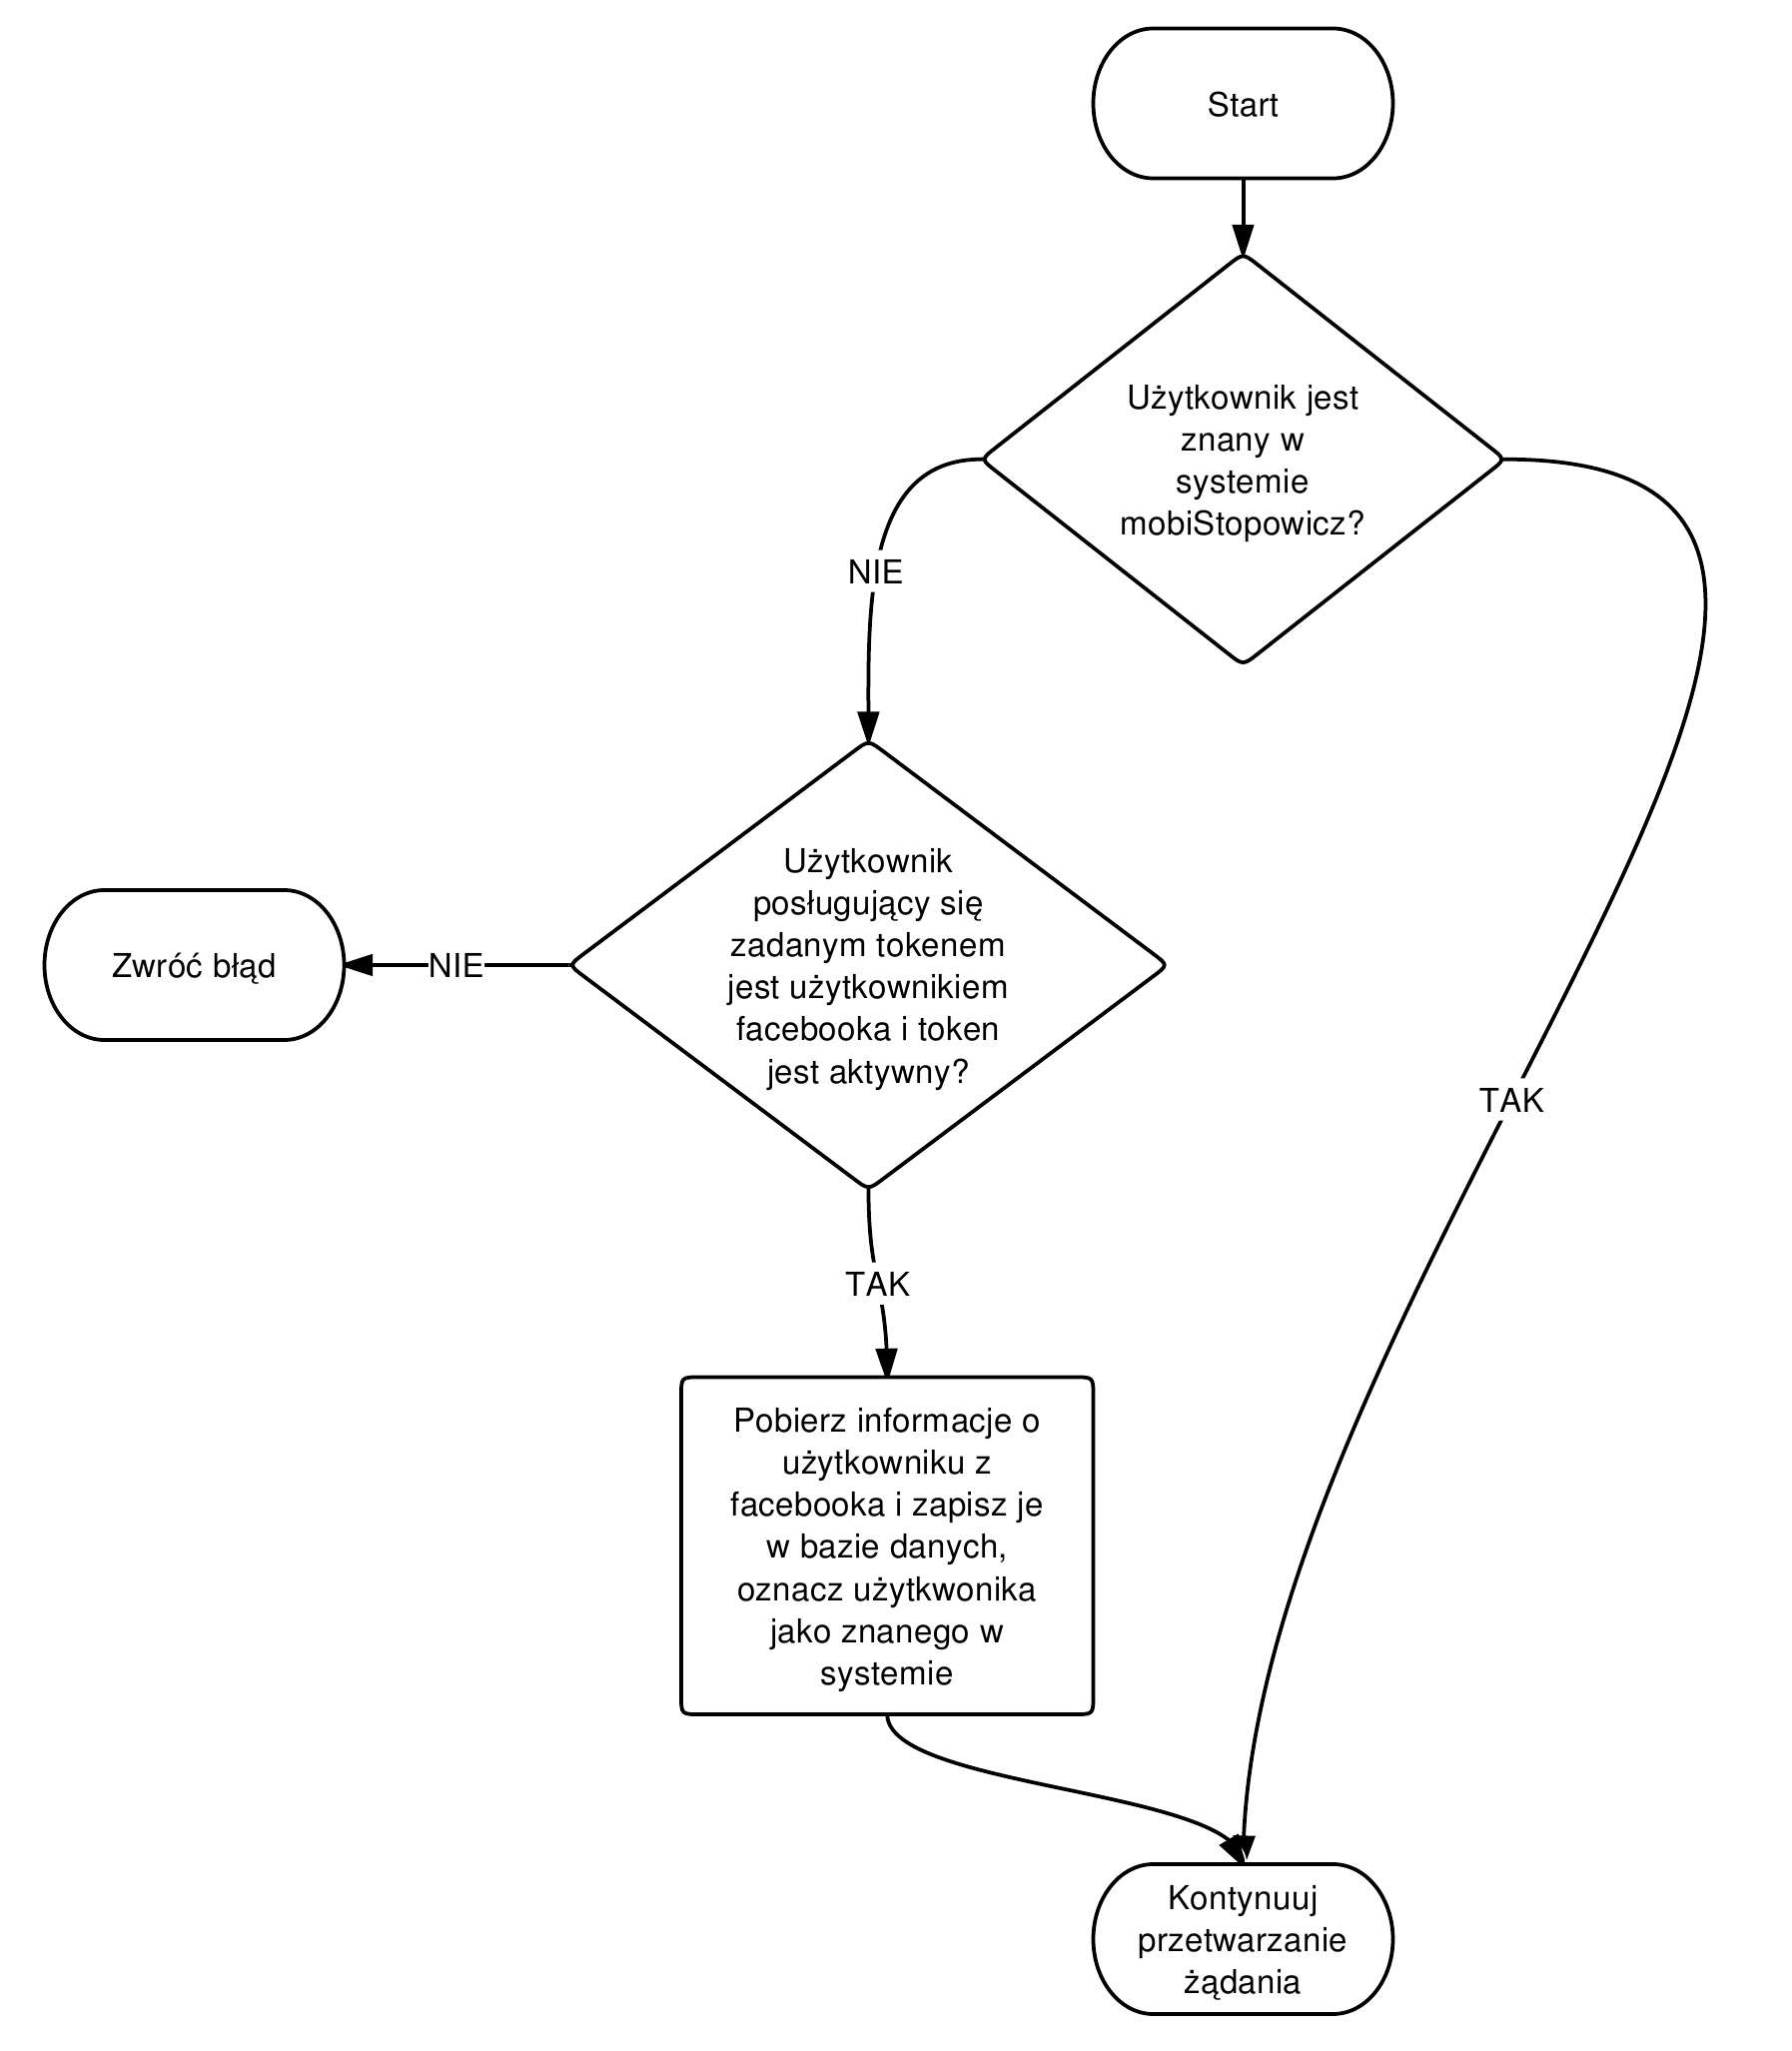
\includegraphics[width=\textwidth]{chap4/img/autentykacja}
	\caption{Pierwsze po��czenie u�ytkownika z serwerem}
	\label{fig:autentykacja}
\end{figure}

\subsection{Obs�uga ��da�}
Ka�de ��danie klienta wysy�ane do serwera mobiStopowicz jest w formacie JSON i zawiera token dost�powy. ��danie klienta jest obs�ugiwane w spos�b przedstawiony na rysunku \ref{fig:obsluga_zadania}
\begin{figure}
	\centering
		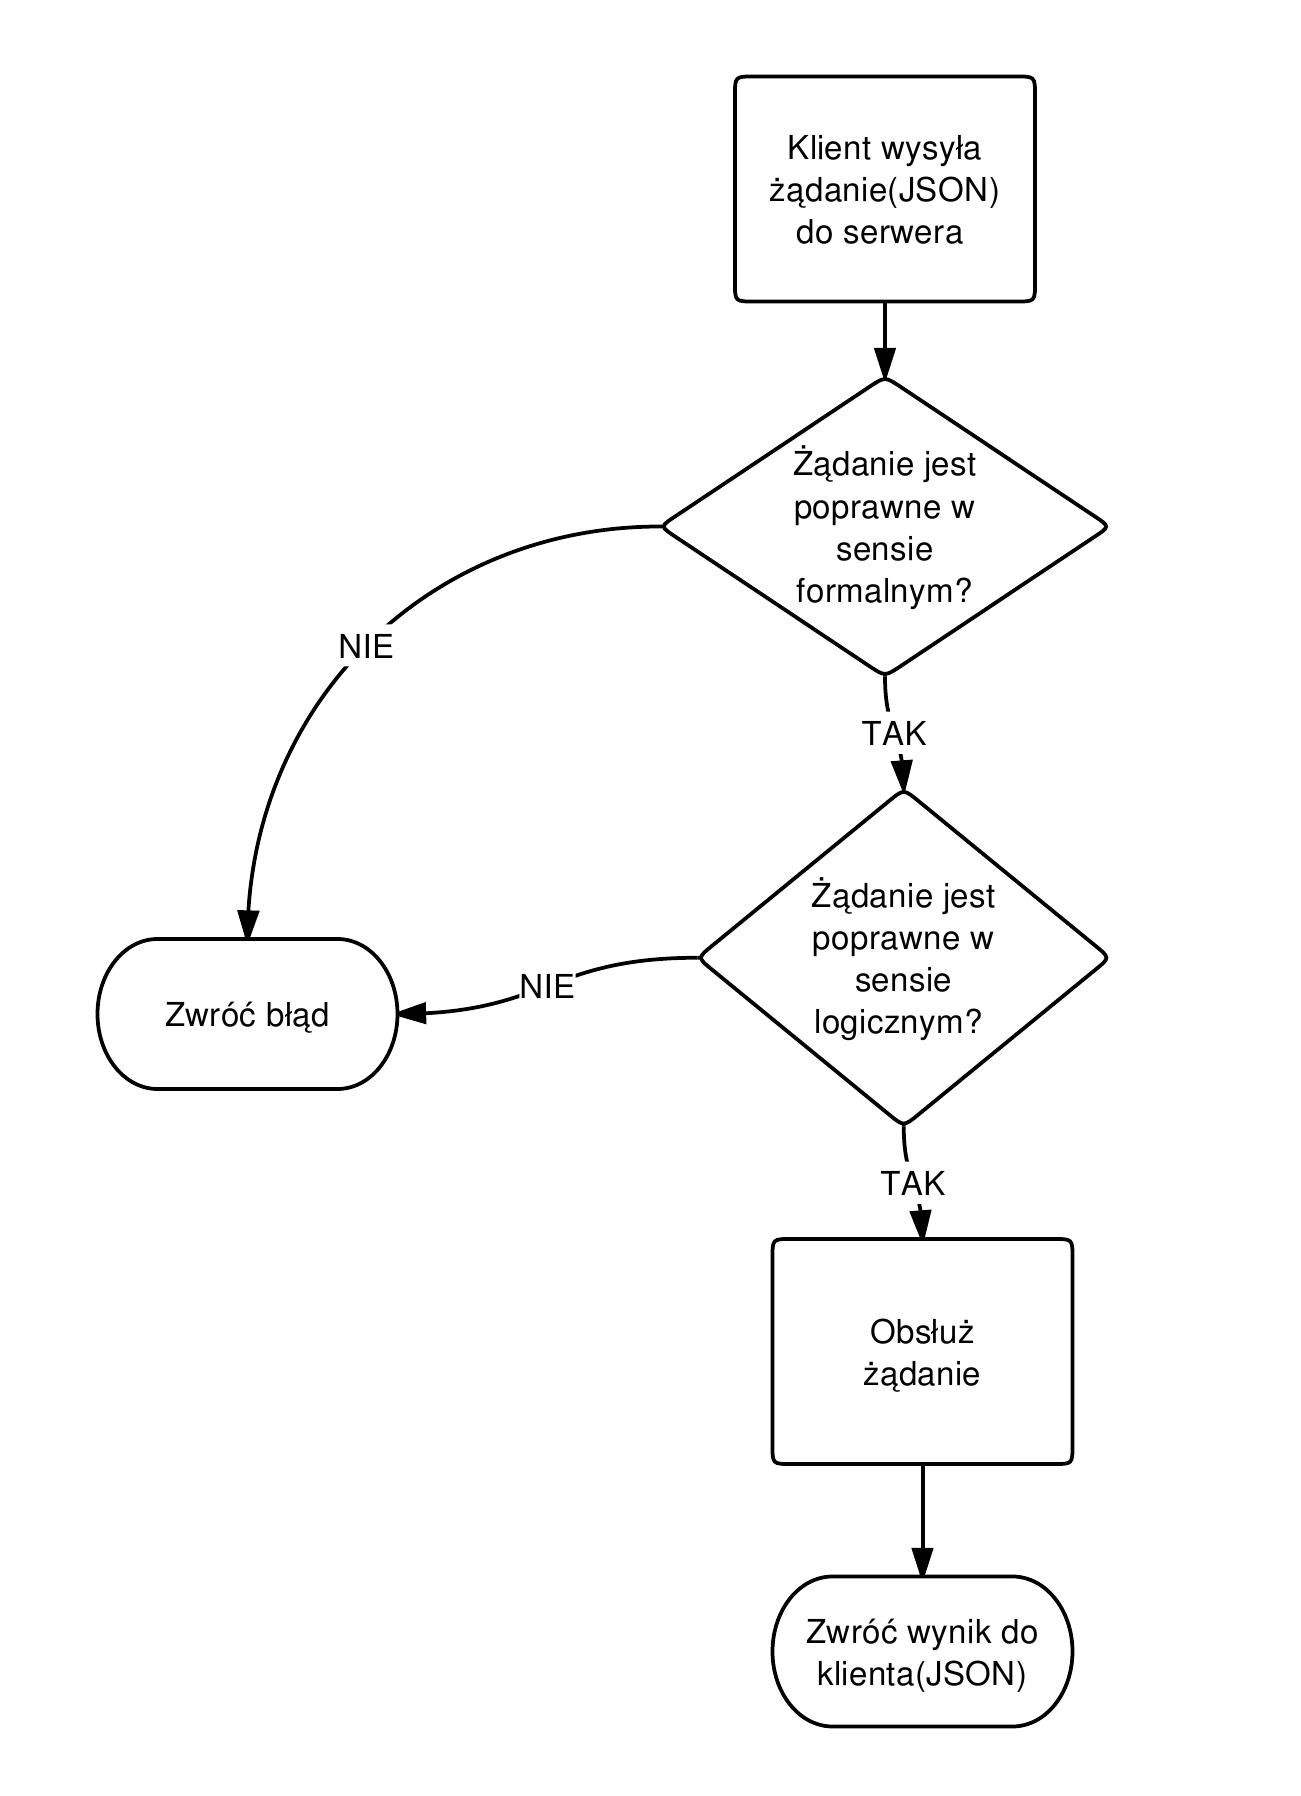
\includegraphics[width=0.70\textwidth]{chap4/img/obsluga_zadania}
		\caption{Przebieg obs�ugi ��dania}
	\label{fig:obsluga_zadania}
\end{figure}

% \chapter{Cz�� programistyczna}
\label{sec:chapter5}

\section{Aplikacja kliencka na platform� BlackBerry}
Aplikacja kliencka jest to komponent systemu mobiStopowicz instalowany na dowolnym urz�dzeniu BlackBerry z systemem operacyjnym 5.0 lub wy�szym. 
\subsection{Platforma BlackBerry}
 \subsubsection{Informacje o platformie}
BlackBerry jest to urz�dzenie typu komputer kieszonkowy z wbudowan� funkcj� telefonu kom�rkowego. Pierwsze urz�dzenie BlackBerry zosta�o wprowadzone w roku 1999. Od samego pocz�tku bardzo du�y nacisk zosta� po�o�ony na obs�ug� poczty elektronicznej. Nowoczesne urz�dzenia BlackBerry obs�uguj� wiadomo�ci e-mail, rozmowy g�osowe, wiadomo�ci tekstowe, przegl�danie sieci WWW i bezprzewodowe us�ugi informacyjne. Pocz�tkowo aplikacje na platform� by�y pisane w j�zyku C++, obecnie wykorzystywany jest j�zyk Java.
 \subsubsection{Przyczyna wyboru platformy}
Platform� BlackBerry wybra�em z kilku powod�w.

\begin{enumerate}
    \item Jest to niezwykle przysz�o�ciowa, a zarazem dojrza�a platforma. W Stanach Zjednoczonych do BlackBerry nale�y ponad 30\% rynku smartphon�w. Tak�e w Polsce urz�dzenia z je�ynk� na obudowie zyskuj� coraz wi�ksz� popularno��.  
    \item System map wraz z geocodingiem jest wbudowany w platform� i dost�pny programowo z poziomu aplikacji, nie trzeba korzysta� z dodatkowych, zewn�trznych, cz�sto p�atnych modu��w.
    \item Ju� wcze�niej zna�em t� platform� i mia�em do�wiadczenia w  pisaniu na ni� aplikacji.
	\item Wszystkie urz�dzenia BlackBerrry s� sprzedawane przez operator�w wraz z us�ug� transmisji danych, kt�ra jest niezb�dna do dzia�ania mojej aplikacji.
\end{enumerate}

\subsection{Funkcje aplikacji}
Aplikacja na platform� BlackBerry jest w pe�ni funkcjonalnym klientem systemu mobiStopowicz i pozwala w ca�o�ci wykorzysta� mo�liwo�ci systemu. A oto najwa�niejsze funkcje aplikacji:

\begin{itemize}
	\item Logowanie do systemu przy u�yciu protoko�u OAuth 2.0 i serwera facebook.com \\
	Obecnie w internecie odchodzi si� od modelu "jeden serwis - jedno konto" na rzecz modelu "wiele serwis�w - jedno konto". W mojej aplikacji zastosowa�em si� do tej zasady i wykorzysta�em publiczny interfejs OAuth udost�pniany przez serwis Facebook. Oznacza to, �e je�li chcemy korzysta� z aplikacji mobiStopowicz wystarczy, �e zalogujemy si� za pomoc� naszego konta na Facebook'u. Jest to nowoczesne i du�o bardziej przyjazne u�ytkownikowi podej�cie. Nie musi on zak�ada� nowego konta, podawa� adresu e-mail i potwierdzi� jego poprawno��, pami�ta� dodatkowego has�a. Jedno logowanie i ju� jest si� u�ytkownikiem serwisu mobiStopowicz.
	\item Dodawanie nowej podr�y (kierowca) \\
	Opcja ta pozwala na dodanie nowej podr�y zaplanowanej przez kierowc�. Dla podr�y musi zosta� okre�lony punkt startu, punkt ko�ca, oraz czas rozpocz�cia. Mo�na poda� dodatkowe parametry okre�laj�ce preferencje co do pasa�er�w. Po utworzeniu podr�y, informacja jest przesy�ana na serwer i staje si� dost�pna dla pasa�er�w.
	\item Wyszukiwanie podr�y (pasa�er) \\
	Opcja ta pozwala na wyszukiwanie podr�y (ofert kierowc�w) przez pasa�era. Mo�e on okre�li� sk�d, dok�d i kiedy chce jecha�. Opcjonalnie mo�e r�wnie� zdefiniowa� dodatkowe kryteria, kt�re zostan� uwzgl�dnione przy poszukiwaniach. Po wys�aniu zapytania na serwer do u�ytkownika zwracana jest lista aktualnie dost�pnych ofert spe�niaj�cych zadane kryteria, b�d� informacja, �e aktualnie nie s� dost�pne �adne oferty.
	\item Do��czenie do istniej�cej podr�y (pasa�er) \\
Pasa�er po znalezieniu oferty spe�niaj�cej jego wymagania ma mo�liwo�� wys�ania ��dania do��czenia do niej. Po zatwierdzeniu, przez kierowc� jego udzia�u zostaje poinformowany o tym, �e uda�o si� do��czy� do podr�y.
   \item Potwierdzenie / odrzucenie ��dania o do��czenie do podr�y (kierowca) \\
Kierowca ma mo�liwo�� zatwierdzi� lub odrzuci� udzia� konkretnego pasa�era w podr�y.
   \item Integracja z facebook.com \\
Aplikacja jest zintegrowana z Facebook'iem. Ka�dy jej u�ytkownik jest r�wnie� u�ytkownikiem Facebook'a. U�ytkownik mo�e obejrze� profil innego u�ytkownika sytemu na Facebook'u, wys�a� mu wiadomo�� oraz korzysta� ze wszystkich innych funkcji udost�pnionych przez serwis.  
	
	
\end{itemize}

\subsection{Wykorzystane biblioteki}
Rozs�dne i umiej�tne wykorzystanie bibliotek jest podstaw� programowania. U�ywanie bibliotek pozwala znacz�co skr�ci� czas pisania aplikacji oraz zwi�ksza jej niezawodno��, poniewa� biblioteki s� zwykle dopracowane i przetestowane przez setki u�ytkownik�w. W mojej aplikacji wykorzysta�em nast�puj�ce biblioteki: 

\subsubsection{Facebook BlackBerry SDK}
Jest to biblioteka typu open source rozpowszechnian� na licencji MIT rozwiajan� przez Eki Y. Baskoro. Biblioteka jest fasad� pozwalaj�c� na korzystanie z protoko��w OAuth 2.0 oraz Graph API udost�pnionych przez Facebook'a. Poniewa� biblioteka jest rozpowszechniana na licencji MIT mia�em mo�liwo�� wyedytowa� kod tak by poprawi� kilka b��d�w oraz dostosowa� go do moich potrzeb.

\subsubsection{org.json}
Biblioteka napisana w j�zyku Java pozwalaj�ca na �atwe manipulowanie obiektami typu JSON. 

\subsubsection{microlog}
Biblioteka s�u��ca do logowania. Dobre i umiej�tne umieszczenie funkcji loguj�cych w aplikacji jest kluczowe aby �ledzi� prac� aplikacji poczas fazy rozwijania. Umiej�tno�� ta jest szczeg�lnie przydatna w przypadku platform mobilnych, gdy cz�sto nie mamy fizycznego (przewodowego) dost�pu do urz�dzenia na kt�rym testowana jest aplikacja.

\subsubsection{imf-blackberry}
Open-sourcowa biblioteka rozwijana przez firm� Polidea. Niezb�dna w fazie testowania aplikacji. Pozwala na zdalne �ledzenie faz �ycia aplikacji, logowanie wyj�tk�w oraz wysy�anie raport�w przez tester�w do programist�w.

\subsubsection{imf-common}
Zestaw klas pomocniczych przeznaczonych na platform� BlackBerry. U�atwia tworzenie i nadzorowanie po��cze� HTTP.


\subsection{Wykorzystane narz�dzia}
Czasy, gdy programy pisano w notatniku a debugowano w konsoli dawno ju� min�y. Obecnie programista ma do dyspozycji szereg narz�dzi u�atwiaj�cych prac�. Ja podczas pisania cz�ci klienckiej korzysta�em z nast�puj�cych narz�dzi:

\subsubsection{Eclipse + BlackBerry Java Plug-in}
Eclipse jest powszechnie znanym �rodowiskiem programistycznym typu IDE (Integrated Development Environment). Eclipse zosta� rozszerzony o plugin BlackBerry Java Plugin pozwalaj�cy na tworzenie i debugowania aplikacji na platform� BlackBerry.

\subsubsection{BlackBerry Smartphone Simulator}
Symulator urz�dzenia BlackBerry �wietnie symuluj�cy zachowanie prawdziwego urz�dzenia. Niezast�piony podczas rozwijania i debuggingu aplikacji.

\begin{figure}[H]
	\centering
		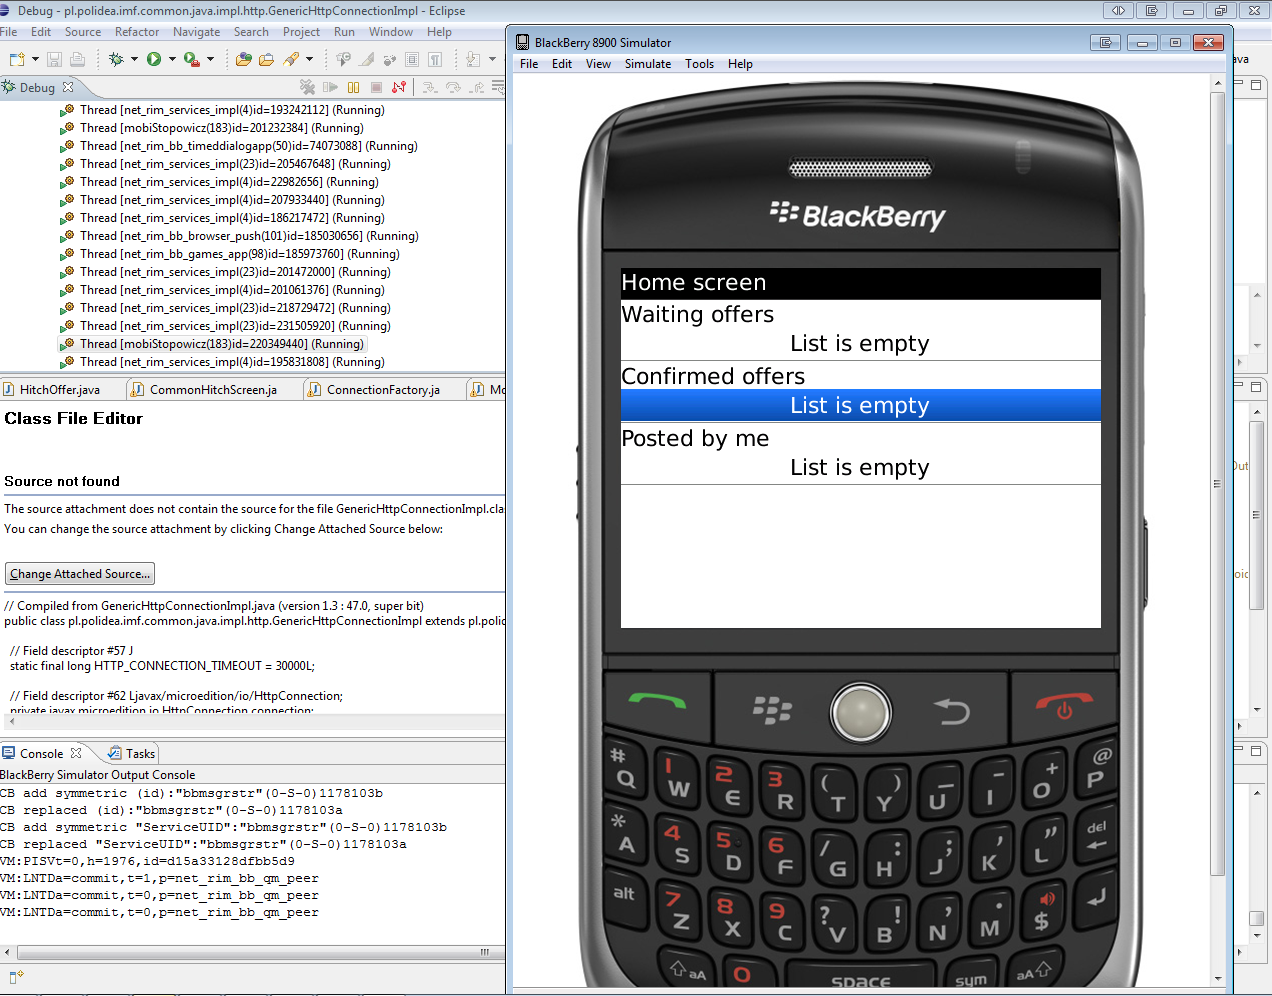
\includegraphics[width=1.00\textwidth]{chap5/screen_env}
	\label{fig:screen_env}
	\caption{Uruchomione �rodowisko Eclipse wraz z emulatorem}
\end{figure}

\subsubsection{Ant}
Narz�dzie do zautomatyzowania procesu budowy oprogramowania. Do opisu procesu budowy oraz zale�no�ci wykorzystywany jest format XML. Podczas rozwijania mojej aplikacji u�ywa�em Ant'a aby zautomatyzowa� proces budowania aplikacji klienckiej oraz zale�nych bibliotek.

\subsubsection{Mercurial}
Jest to rozproszony, mi�dzyplatformowy system kontroli wersji. Mercurial cechuje si� du�� wydajno�ci�, skalowalno�ci� i rozproszono�ci�. Pozwala na tworzenie lokalnych repozytori�w jak i korzystanie ze zdalnych. Podczas mojej pracy by� niezast�pionym narz�dziem do zarz�dzania wersjami kodu. 

\begin{figure}[h]
	\centering
		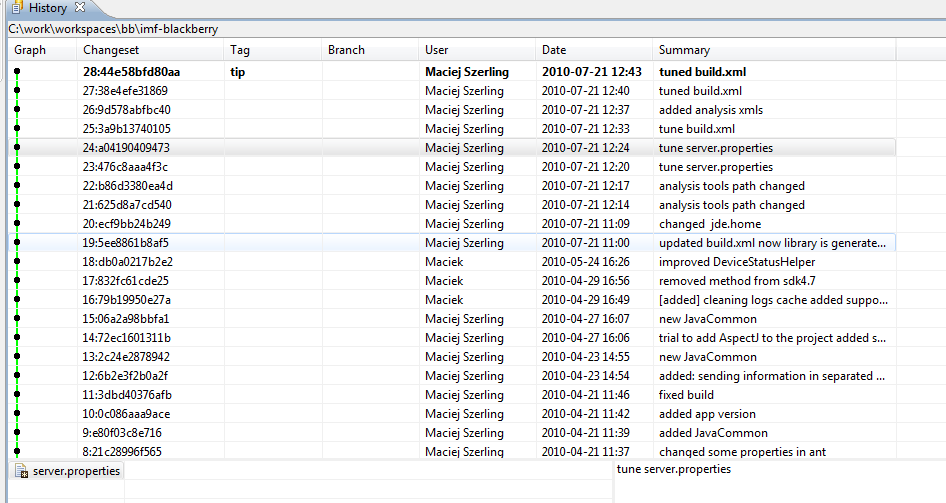
\includegraphics[width=1.00\textwidth]{chap5/screen_hg}
	\label{fig:screen_hg}
	\caption{System kontroli wersji w dzia�aniu}
\end{figure}

\subsection{Implementacja}
Aplikacja kliencka zosta�a napisana obiektowo w j�zyku Java. Aplikacja zosta�a napisana zgodnie z wzorcem architektonicznym MVC(Model-View-Controller)
\subsection{Testy}
Tworzone oprogramowanie, podobnie jak wszystkie produkty na rynku, musi posiada� odpowiedni� jako��, aby by�o atrakcyjne dla odbiorc�w. Najwa�niejszym i podstawowym sposobem zapewnienia jako�ci oprogramowania s� testy. B��dy w oprogramowaniu wyst�puj� zawsze, a ich �r�de� jest wiele. Testy pozwalaj� na ich mo�liwie szybkie wykrycie i wyeliminowania. Im szybciej b��d zostanie wykryty tym mniejszy jest koszt jego usuni�cia.
\subsubsection{Testy jednostkowe}
Testy jednostkowe (Unit tests) s� metod� testowania oprogramowania polegaj�c� na wykonywaniu test�w weryfikuj�cych poprawno�� dzia�ania pojedynczych, najmniejszych, niepodzielnych jednostek aplikacji. Testowany fragment programu poddawany testowi jest wykonywany, a wynik przez niego zwr�cony por�wnywany jest z wynikiem oczekiwanym. Wielk� zalet� test�w jednostkowych jest mo�liwo�� wykonywania test�w na modyfikowanych jednostkach programu i wykrycie b��du zaraz po jego pojawieniu.

W aplikacji mobiStopowicz testy jednostkowe wykonywa�em manualnie, testuj�c konkretne modu�y aplikacji. W wyniku test�w jednostkowych zosta�o wykryte wiele pomniejszych b��d�w, kilka powa�niejszych oraz jeden krytyczny zwi�zany ze z�� obs�ug� b��d�w.
\subsubsection{Testy funkcjonalne}
W testach funkcjonalnych testowany program traktowany jest jak czarna skrzynka, kt�rej wn�trze nie jest znane testerowi. Tester sprawdza zgodno�� aplikacji z za�o�eniami funkcjonalnymi znajduj�cymi si� w dokumentacji.

Testy funkcjonalne aplikacji klienckiej mobiStopowicz by�y przeprowadzana przeze mnie, a tak�e przez niezale�nego testera.
W wyniku test�w zosta� wykryty jeden powa�ny b��d polegaj�cy na niezgodno�ci zachowania aplikacji z za�o�eniami funkcjonalnymi.

\section{Aplikacja serwerowa oparta o GAE}
Wyb�r technologii, w kt�rej powstanie aplikacja serwerowa, sprawi� mi do�� wiele problemu. Pocz�tkowo zdecydowa�em si� na u�ycie rozwi�zania dostarczanego przez firm� Microsoft a mianowicie .NET i jego webowa cze�� ASP.NET. Zrezygnowa�em jednak z jego u�ycia z kilku powod�w:
\begin{enumerate}
	\item Wiele niezb�dnych bibliotek pod platform� .NET jest p�atnych, nie s� nawet dost�pne darmowe wersje do cel�w edukacyjnych.
	\item Musia�bym dysponowa� zewn�trznym serwerem pozwalaj�cym na hostowanie aplikacji ASP.NET, kt�ry r�wnie� jest p�atny.
	\item Cz�� kliencka aplikacji mia�a powsta� w j�zyku Java, natomiast w .NET u�ywany jest c\# z tego powodu pewne prace integracyjne wymaga�y by wi�kszego nak�adu pracy.
\end{enumerate}
Nast�pnie postanowi�em, �e cz�� serwerowa powstanie w Pythonie. Jest to niezwykle efektywny i bardzo pr�nie rozwijaj�cy si� j�zyk, jednak ostatecznie zosta� przeze mnie odrzucony. Podobnie jak w przypadku .NET zawa�y� fakt, i� aplikacja kliencka powstaje w j�zyku Java i nak�ad prac integracyjnych b�dzie do�� znaczny.

Ostatecznie wybra�em j�zyk Java i platform� Java EE. By�a ona pozbawiona wad powy�szych rozwi�za�, dodatkowo skorzysta�em z darmowych us�ug hostingowych firmy Google, co wyeliminowa�o konieczno�� uruchamiania w�asnego serwera b�d� wykupowania p�atnych us�ug hostingowych.
 
\subsection{Platforma Google App Engine}

 \subsubsection{Informacje o platformie}
 GAE (Google App Engine) jest to platforma przeznaczona do tworzenia i hostowania skalowalnych aplikacji webowych udost�pniona do publicznego u�ytku w 2008r. przez firm� Google. GAE pozwala na tworzenie aplikacji w j�zyku Java oraz Python. 
 \subsubsection{Przyczyna wyboru platformy}
	Platforma Google App Engine wykorzystuj�ca Jav� EE zosta�a wybrana przeze mnie z kilku powod�w:
	
\begin{enumerate}
	\item Do GAE dostarczone jest �rodowisko programistyczne oparte o program Eclipse, kt�re w znacznym stopniu u�atwia proces pisania aplikacji.
	\item Hosting aplikacji jest darmowy.
	\item Cz�� serwerowa jest napisana w tym samym j�zyku co cz�� kliencka, z tego powodu nak�ad prac integracyjnych jest znacznie mniejszy, ni� w przypadku rozwi�za� pisanych w r�nych j�zykach.
\end{enumerate}
\subsection{Funkcje}
API (Application Programming Interface) strony serwerowej pozwala przeprowadzi� nast�puj�ce akcje:
\begin{itemize}
	\item Wyszukaj oferty podr�y dla warunk�w zadanych przez podr�nego \\
	Ta funkcja serwera pozwala na wyszukanie ofert podr�y zg�oszonych przez kierowc�w spe�niaj�cych warunki zadane przez podr�nego.
	\item  Dodaj ofert� kierowcy \\
	Ta funkcja serwera pozwala na dodanie nowej oferty kierowcy do systemu.
	\item Wy�lij ��danie do��czenia do podr�y \\
	Pozwala podr�nemu do��czy� do konkretnej podr�y.
	\item Zatwierd� pro�b� o do��czenie do podr�y \\
	Pozwala kierowcy zaakceptowa� pro�b� pasa�era do do��czenia do jednej z ofert wys�anych przez kierowc�.
	
	
\end{itemize}
\subsection{Wykorzystane biblioteki}
\subsubsection{javageomodel}
Niezwykle ciekawa biblioteka. Jeden z g��wnych filar�w aplikacji serwerowej. Biblioteka pozwala por�wnywa� punkty na p�aszczy�nie w spos�b liniowy. Aby wyja�ni� spos�b dzia�ania biblioteki nale�y na pocz�tku zdefiniowa� czym jest geocell:

Geocell - jest to heksadecymalny ci�g znak�w kt�ry okre�la dwuwymiarowy prostok�tny obszar wewn�trz przestrzeni szerkoko�� / d�ugo�� geograficzna [-90, 90] x [-180, 180]. Rozdzielczo�� geocell'a jest okre�lona przez d�ugo�� ci�gu znak�w. Geocell'e o wysokiej rozdzielczo�ci z praktycznego punktu widzenia mog� by� traktowane jako punkty.

Aby wyznaczy� prostok�t odpowiadaj�cy konkretnemu geocell'owi w pierwszym kroku przestrze� [-90, 90] x [-180, 180] dzielona jest na siatk� 4 x 4:

\begin{verbatim}
                 +---+---+---+---+ (90, 180)
                 | a | b | e | f |
                 +---+---+---+---+
                 | 8 | 9 | c | d |
                 +---+---+---+---+
                 | 2 | 3 | 6 | 7 |
                 +---+---+---+---+
                 | 0 | 1 | 4 | 5 |
      (-90,-180) +---+---+---+---+
\end{verbatim}

w nast�pnym kroku du�e prostok�ty, dzielone s� na mniejsze i rozdzielczo�� geocell'i si� zwi�ksza. W przypadku geocella '7' kolejny podzia� b�dzie wygl�da� nast�puj�co:
\begin{figure}[H]
\begin{verbatim}
                                   .                   .
                   .                   .
               . . +----+----+----+----+ (0, 180)
                   | 7a | 7b | 7e | 7f |
                   +----+----+----+----+
                   | 78 | 79 | 7c | 7d |
                   +----+----+----+----+
                   | 72 | 73 | 76 | 77 |
                   +----+----+----+----+
                   | 70 | 71 | 74 | 75 |
      . . (-45,90) +----+----+----+----+
                   .                   .
                   .                   .
\end{verbatim}
\end{figure}

Kolejne kroki polegaj� na dzieleniu przestrzeni na coraz mniejsze prostok�ty do momentu osi�gni�cia geocell'i w postaci string�w pe�nej d�ugo�ci.

Przy u�yciu geocell'i ka�demu punktowi na ziemi przypisujemy prostok�t w kt�rym si� on znajduje, oraz ci�g znak�w jednoznacznie okre�laj�cy ten prostok�t. Punkty znajduj�ce si� blisko siebie w olbrzymiej wi�kszo�ci przypadk�w, maj� bardzo podobne do siebie prefiksy. Wyszukuj�c kilka punkt�w z prefiksem zgadzaj�cym si� na N pozycjach jeste�my w stanie wyszuka�, z zadan� dok�adno�ci�, punkty znajduj�ce si� blisko siebie.

\subsubsection{google-gson} 
Gson jest bibliotek� przeznaczon� dla j�zyka Java pozwalaj�ca na �atw� konwersj� obiekt�w Java Objects do ich reprezentacji w postaci JSON. Pozwala ona r�wnie� na konwersj� obiekt�w JSON w postaci �a�cuch�w znak�w do odpowiadaj�cym im obiektom j�zyka Java. 

W mojej aplikacji Gson zosta� u�yty do konwertowania obiekt�w przesy�anych przez aplikacj� klienck� do serwera do obiekt�w j�zyka Java, a nast�pnie, przy tworzeniu odpowiedzi, obiekty j�zyka Java by�y konwertowane do ich reprezentacji JSON w postaci �a�cucha znak�w r�wnie� przy wykorzystaniu tej biblioteki.

\subsection{Wykorzystane narz�dzia}
\subsubsection{Eclipse + Google Plugin for Eclipse}
Podczas mojej pracy wykorzysta�em IDE Eclipse wraz z do��czonym plugin'em Google Plugin for Eclipse, kt�ry pozwoli� mi w �atwy spos�b tworzy�, rozwija� oraz debugowa� aplikacje przeznaczone na platform� Google App Engine. �rodowisko zawiera wbudowany, testowy serwer http oparty o serwer Jetty.
\subsubsection{JUnit}
Jest to narz�dzie do tworzenia i uruchamiania test�w jednostkowych oprogramowania napisanego w j�zyku Java. W mojej pracy wykorzysta�em je jako narz�dzie wspieraj�ce proces testowania.

\subsection{Implementacja}
Cz�� serwerowa, podobnie jak cz�� kliencka zosta�a napisana w j�zyku Java. Do obs�ugi ��da� zosta� wykorzystany standardowy mechanizm servlet'�w. Aplikacja ma wyra�nie wydzielone komponenty zgodne z architektur� MVC.

\subsection{Metody testowania}
Podobnie jak cz�� kliencka, cz�� serwerowa zosta�a intensywnie przetestowana w celu zapewnienia wysokiej jako�ci aplikacji. Zosta�y przeprowadzone testy jednostkowe przy wykorzystaniu biblioteki JUnit, oraz szereg test�w funkcjonalnych.
\subsubsection{Testy jednostkowe}
Testy jednostkowe zosta�y wykorzystane, aby przetestowa� czy poszczeg�lne, najmniejsze modu�y aplikacji dzia�aj� poprawnie. Testami zosta�y pokryte:
\begin{itemize}
	\item Operacje wstawiania, modyfikowania i usuwania danych z bazy danych.
	\item Operacje przygotowywania odpowiedzi do klienta, zgodno�� z ustalonym formatem.
	\item Zachowanie logiki aplikacji.
	\item Algorytm parowania kierowc�w i pasa�er�w do wsp�lnej podr�y.
\end{itemize}

W wyniku test�w jednostkowych zosta�o wykrytych kilka b��d�w podczas manipulacji na danych, b��d formatu odpowiedzi dla klienta, oraz jeden powa�ny b��d w algorytmie.
\subsubsection{Testy funkcjonalne}
Testy funkcjonalne zosta�y przeprowadzone przeze mnie, oraz jednego, niezale�nego testera nieznaj�cego wewn�trznej budowy aplikacji. Testy by�y przeprowadzone po�rednio przy wykorzystaniu aplikacji klienckiej, a ruch na ��czu klient-serwer by� monitorowany i por�wnywany z oczekiwanym. W wyniku test�w funkcjonalnych nie zosta�y wykryte �adne znacz�ce b��dy.


\section{Integracja aplikacji klienckiej oraz aplikacji serwerowej}
Integracja cz�ci klienckiej oraz serwerowej by�a przeprowadzana w kilku krokach.
\begin{enumerate}
	\item Przetestowanie, czy zar�wno cz�� serwerowa oraz kliencka przestrzega ustalonego protoko�u komunikacyjnego.
	\item Utworzenie lokalnego �rodowiska testowego.
	\item Uruchomienie aplikacji klienckiej oraz aplikacji serwerowej w �rodowisku testowym.
	\item Iteracyjne testy wsp�pracy oraz naprawa b��d�w do momentu uzyskania rozwi�zania w pe�ni dzia�aj�cego.
	\item Przygotowania �rodowiska zdalnego.
	\item Uruchomienia aplikacji klienckiej oraz aplikacji w �rodowisku zdalnym.
	\item Alpha testy w �rodowisku zdalnym.
	
\end{enumerate}
\subsection{Interfejs komunikacyjny}
Interfejs komunikacyjny mi�dzy aplikacj� klienck� jest niezwykle prosty, a zarazem efektywny i rozszerzalny. Klient komunikuje si� z serwerem przy u�yciu metod opisanych w tabeli \ref{tab:interfejsKomunikacyjny}.
\begin{table}[h]
	\centering
		\begin{tabular}{| l | l | }
		  \hline
			Metoda & Funkcja \\ \hline
			addTravelRequest & Umo�liwia wys�anie zapytania o oferty kierowc�w przez pasa�era. \\ \hline
			addTravelOffer & Umo�liwia wys�anie nowej oferty przez kierowc�. \\ \hline
			joinTravel & Pozwala pasa�erowi do��czy� do oferty kierowcy. \\ \hline
			acceptJoin & Pozwala zaakceptowa� kierowcy udzia� pasa�era w podr�y. \\ \hline
			keepAlive & Metoda wykorzystywana do dowiadywania si� o zmianach na serwerze. \\ \hline
			
			
		\end{tabular}
	\caption{Metody interfejsu komunikacyjnego}
	\label{tab:interfejsKomunikacyjny}
\end{table}
\subsection{�rodowisko testowe}
W celu testowania aplikacji zosta�y zestawione dwa �rodowiska testowe. Jedno w pe�ni wirtualne, drugie z wykorzystaniem prawdziwego urz�dzenia typu BlackBerry.
\subsubsection{�rodowisko lokalne (lokalny GAE + Symulator BlackBerry)}
Jest to �rodowisko, w kt�rym by�y przeprowadzane pierwsze testy. Wszystkie elementy, opr�cz serwera Facebook'a s� uruchomione lokalnie na komputerze klasy PC pod kontrol� systemu Windows 7.

\begin{figure}[H]
	\centering
		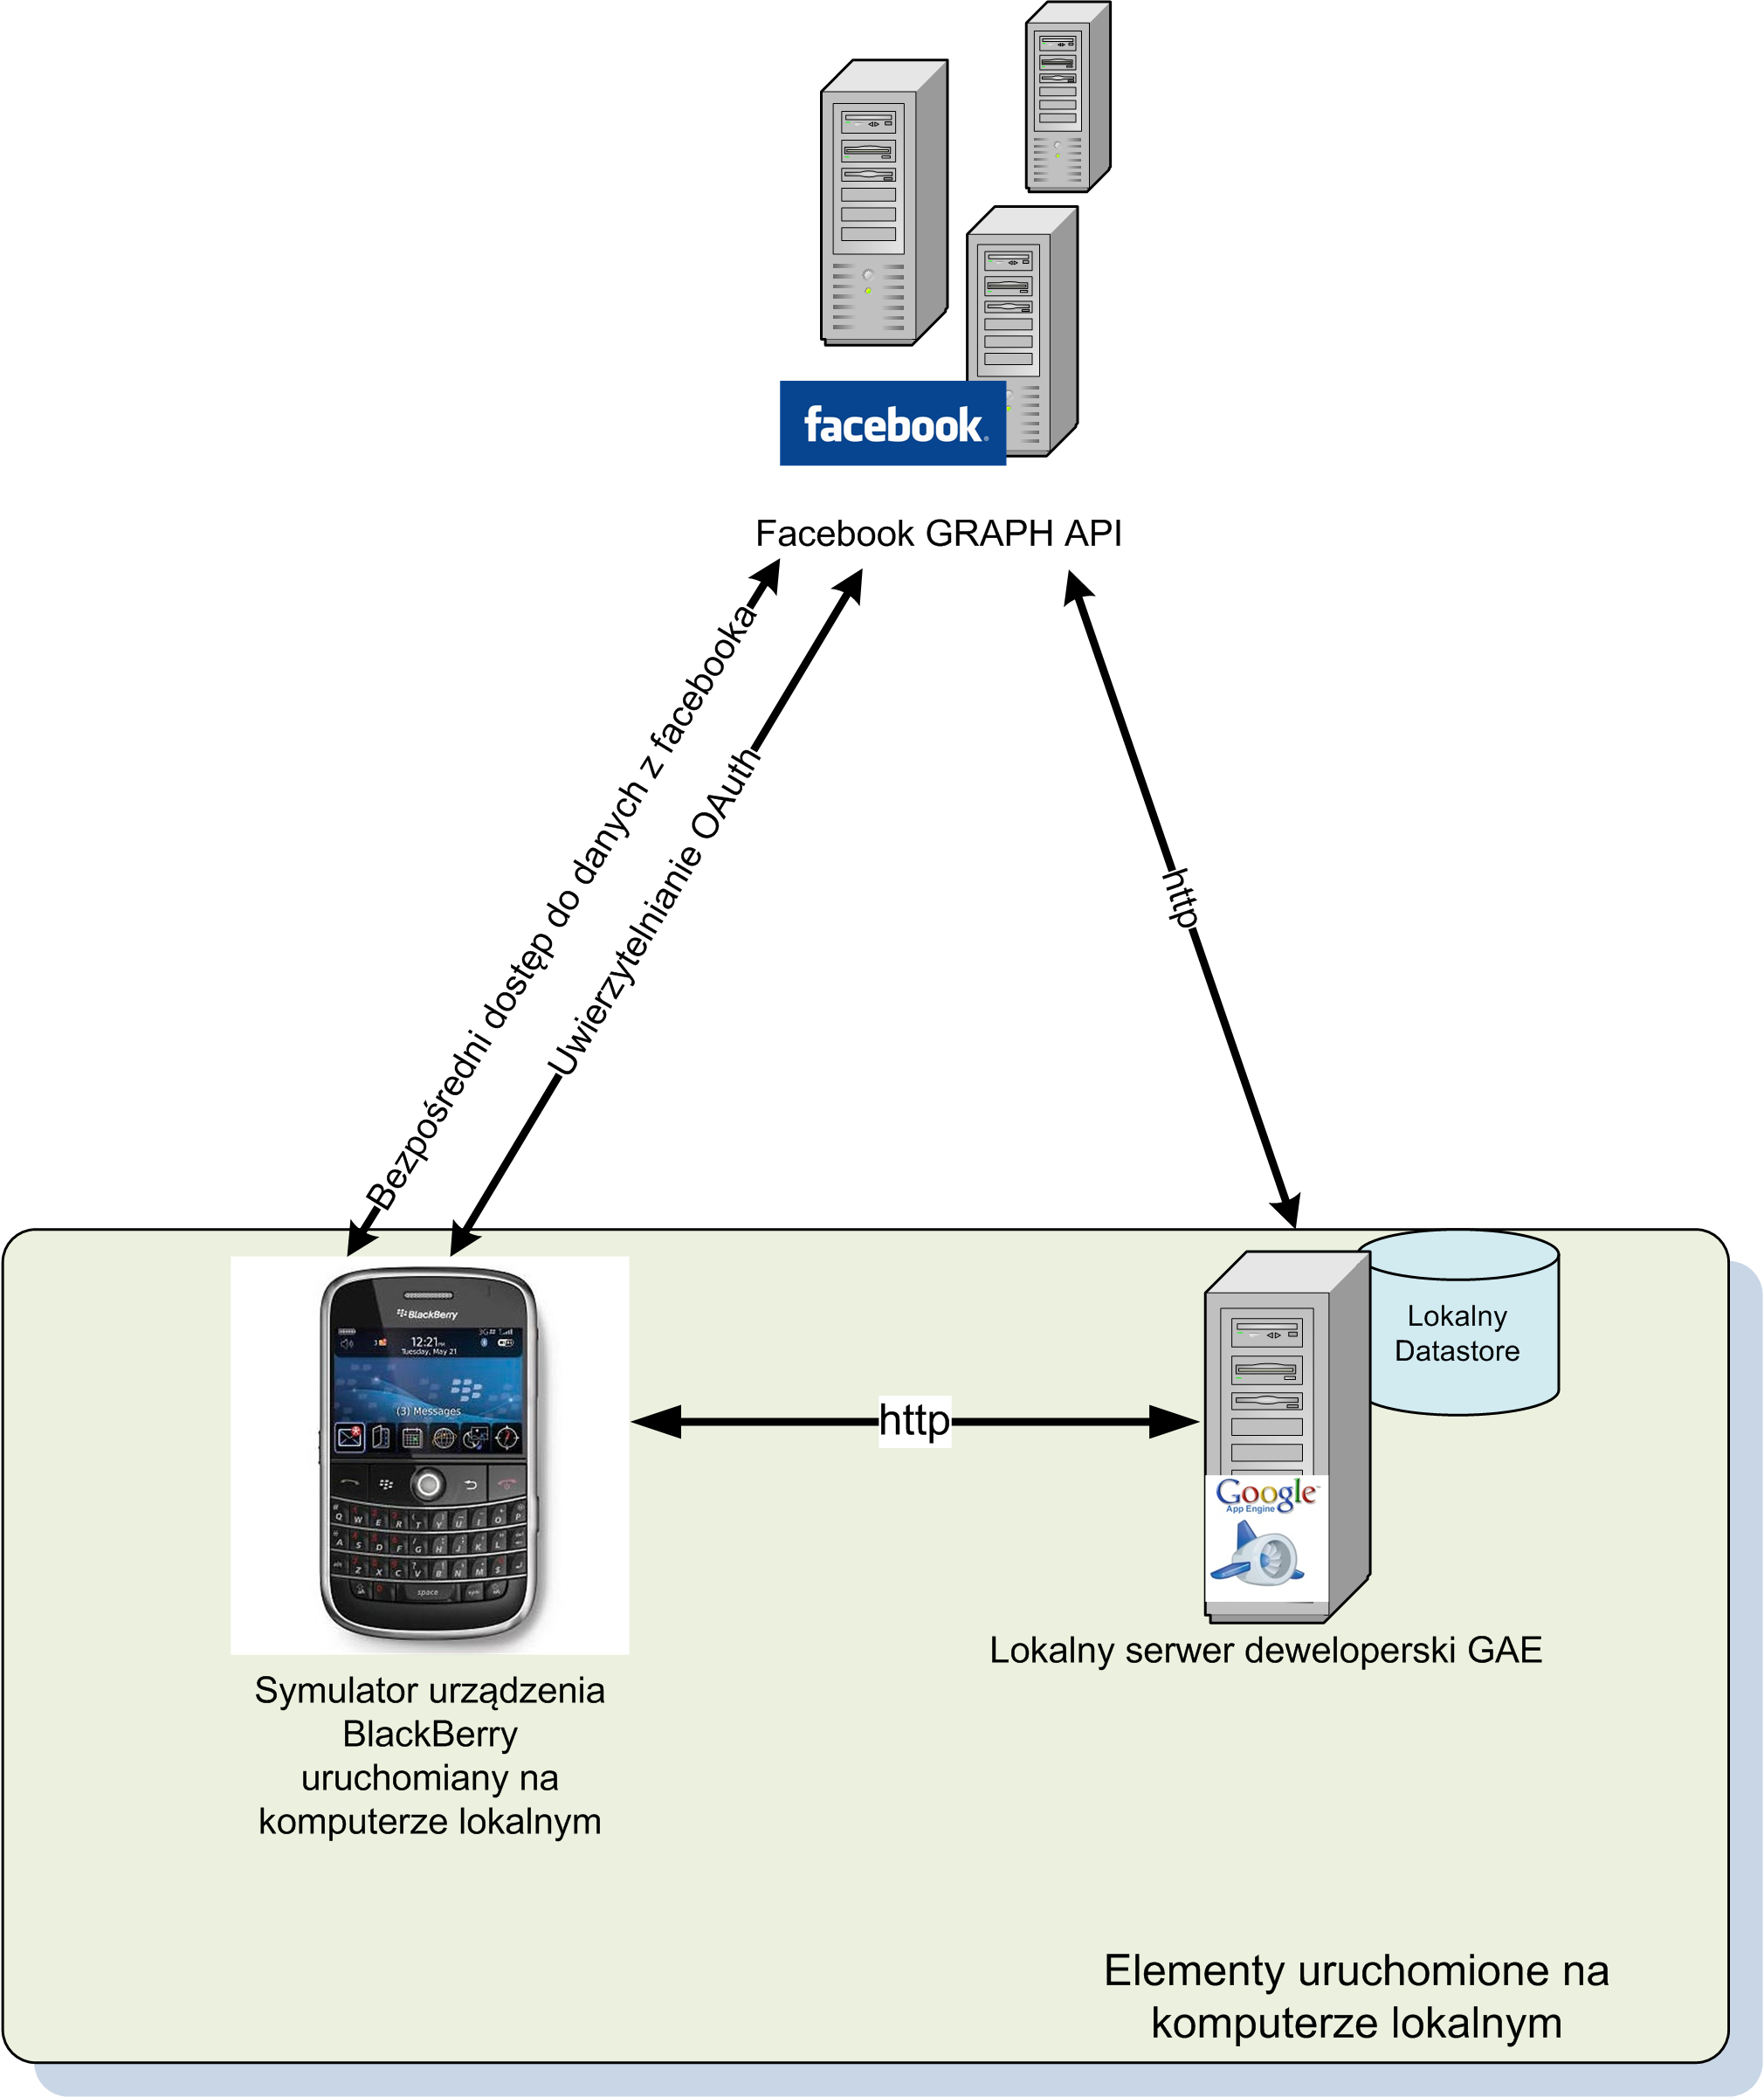
\includegraphics[width=0.70\textwidth]{chap5/srodowisko_testowe_1}
	\caption{Lokalne �rodowisko testowe}
	\label{fig:srodowisko_testowe_1}
\end{figure}

\subsubsection{�rodowisko live (zdalny GAE + rzeczywiste urz�dzenie BlackBerry)}
�rodowisko live zosta�o zestawione w p�niejszym etapie test�w. Aplikacj� uruchomiono na rzeczywistym urz�dzeniu BlackBerry 9500. Aplikacja serwerowa zosta�a zamieszczona i uruchomione w chmurze serwer�w Google'a.
\begin{figure}[H]
	\centering
		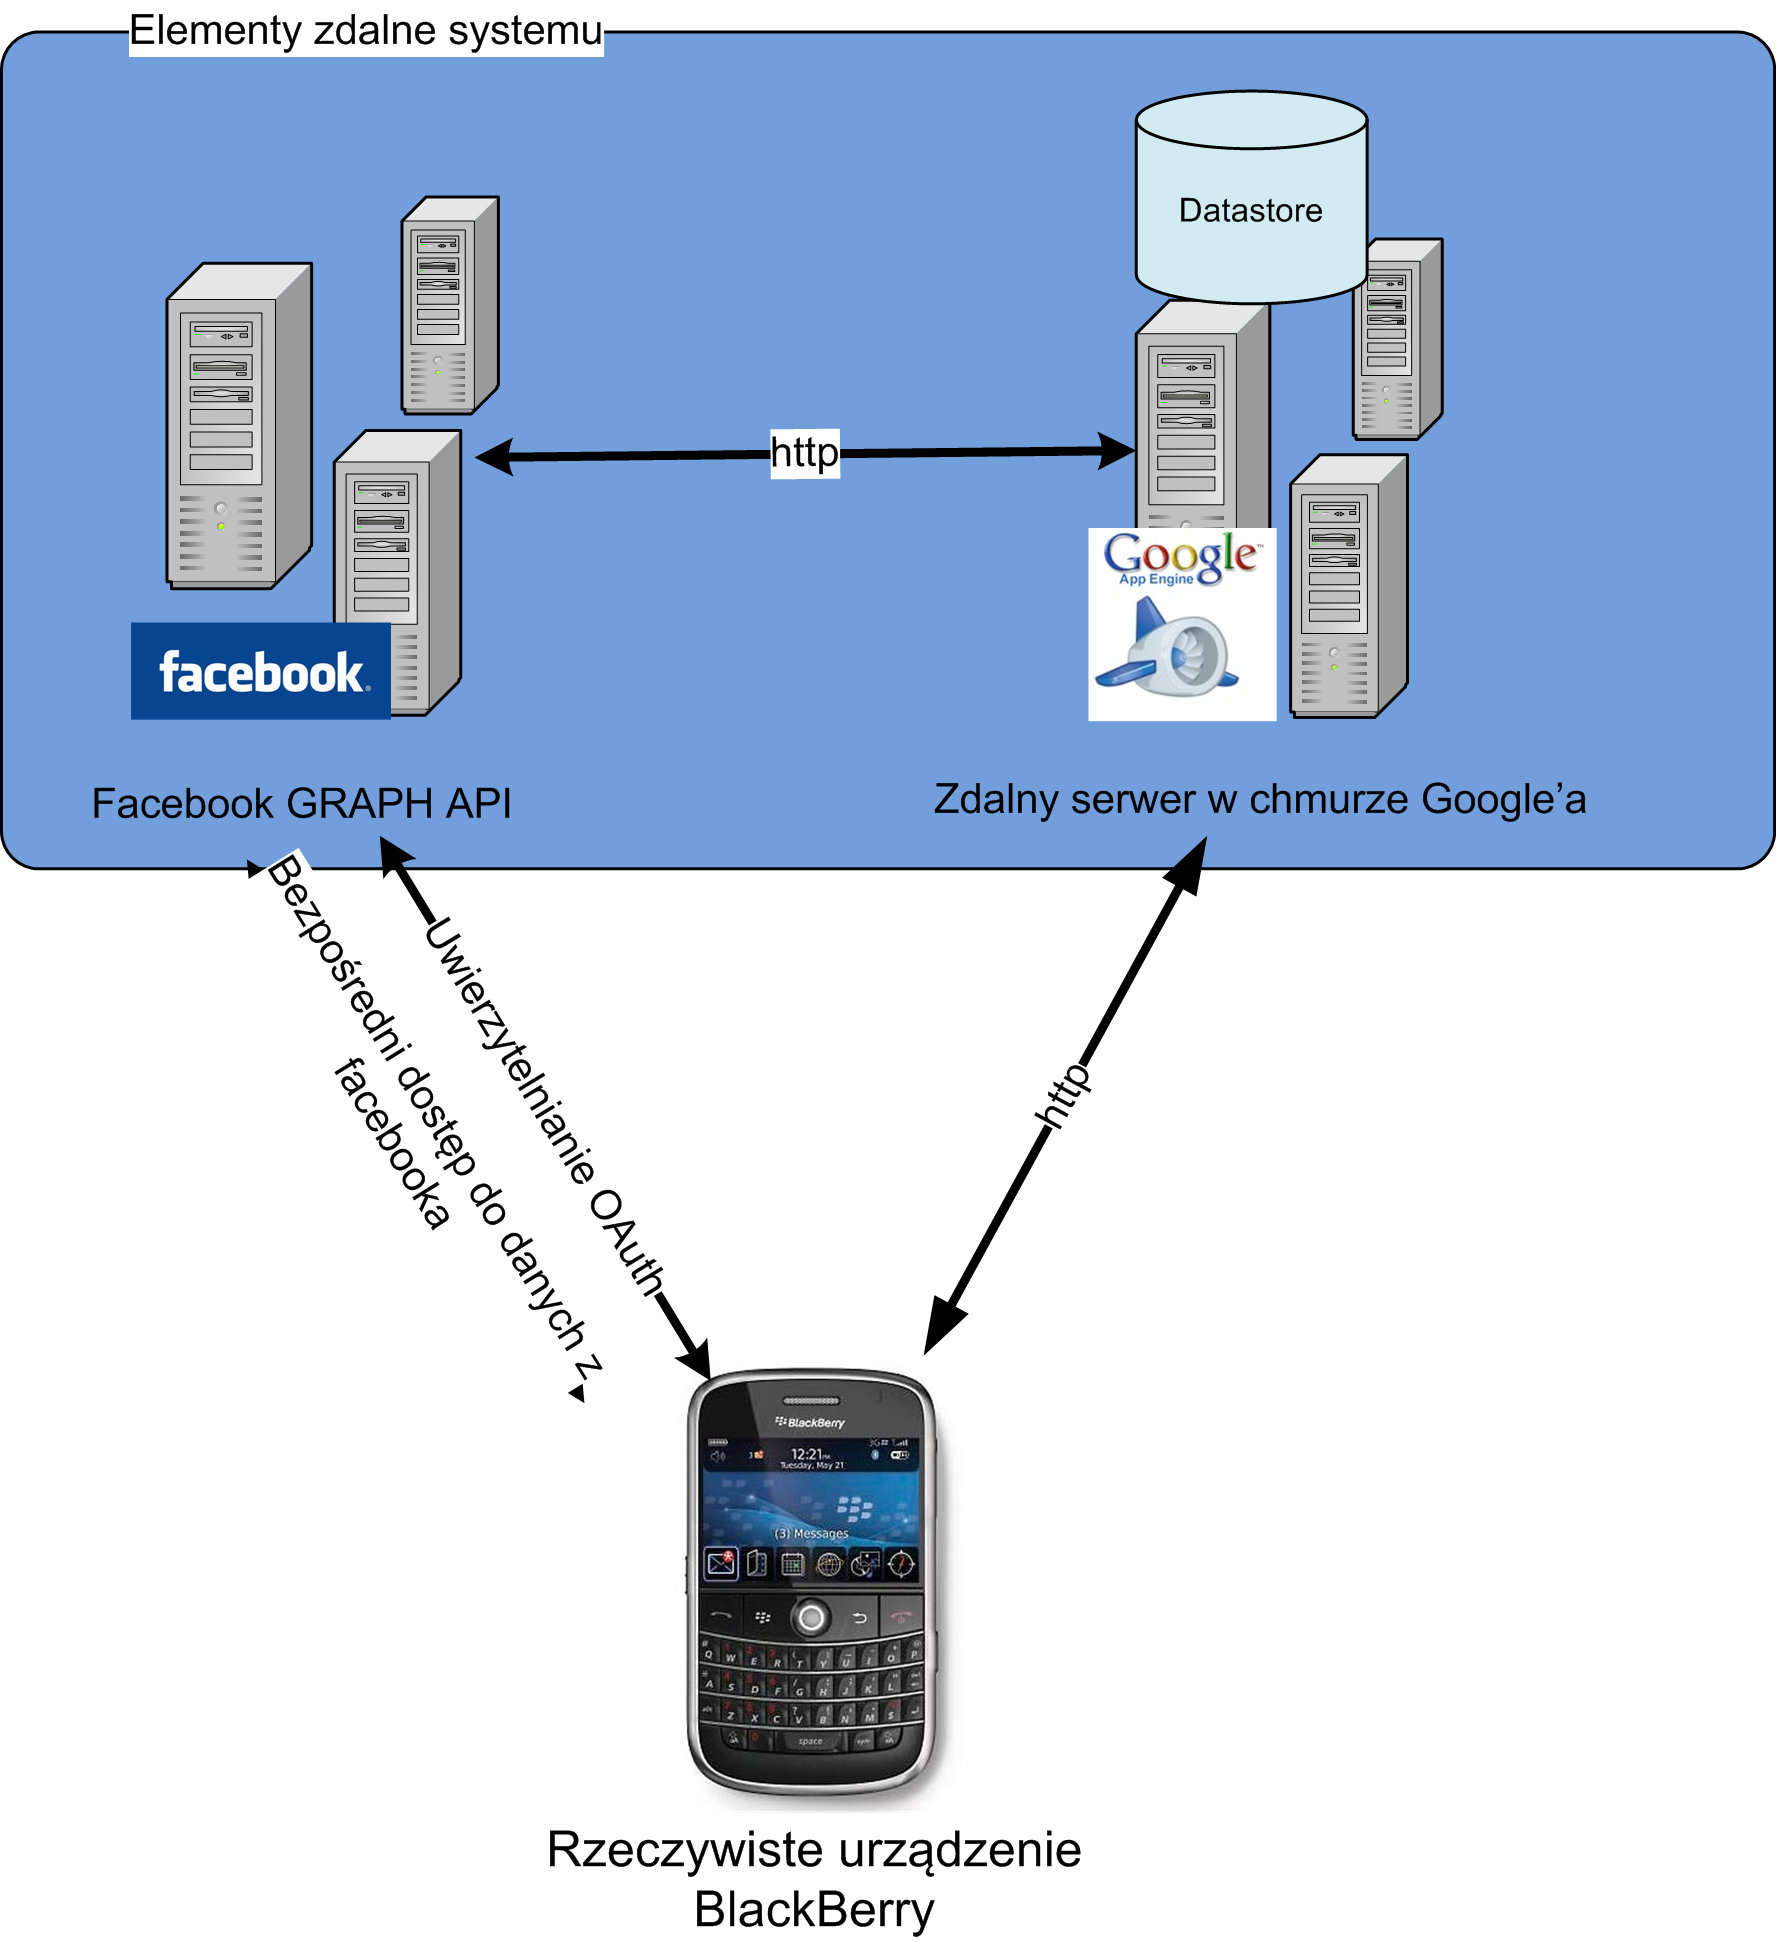
\includegraphics[width=0.70\textwidth]{chap5/srodowisko_testowe_2}
	\caption{�rodowisko testowe typu "live"}
	\label{fig:srodowisko_testowe_1}
\end{figure}


% \chapter{Podsumowanie i perspektywy wdro�enia systemu}
\label{sec:chapter6}

\section{Zrealizowane cele}
W tym punkcie postaram si� sprawdzi� jak cele postawione na wst�pie maj� si� do tego, co uda�o mi si� osi�gn��. Przypomnijmy wi�c postawione we wst�pie cele:

\begin{itemize}
    \item Jasne okre�lenie sk�d, dok�d i kiedy chcemy dojecha�. \\
    Cel zosta� w pe�nie zrealizowany.
    \item Zweryfikowanie to�samo�ci zar�wno kierowcy jak i pasa�era. \\
    Dzi�ki integracji z Facebook'iem mamy mo�liwo�� weryfikowa� to�samo�ci u�ytkownik�w przez ich publiczny profil oraz kontekst w jakim wyst�puje.
    \item Sparowanie pasa�era oraz kierowcy zar�wno z du�ym wyprzedzeniem jak i Ad hoc w czasie rzeczywistym. \\
    System jest zdolny dokonywa� parowa� zar�wno z du�ym wyprzedzeniem, jak i w przypadku podr�y odbywaj�cych si� "za 5 minut".
	  \item System jest skalowalny i globalny, b�dzie w stanie obs�u�y� du�e ilo�ci u�ytkownik�w na ca�ym �wiecie. \\
	  Dzi�ki wykorzystaniu algorytmu parowania o z�o�ono�ci liniowej oraz skalowalnej platformy hostingowej Google App Engine powsta�y system jest skalowalny i gotowy na obs�ug� du�ej ilo�ci u�ytkownik�w.
    \item System jest �atwo rozszerzalny o nowe platformy klienckie (Android, iPhone, etc.) \\
    Interfejs serwera zosta� tak zaprojektowany, �e do��czenie kolejnej platformy klienckiej nie b�dzie stanowi�o �adnego problemu. �aden z element�w serwera nie jest zale�ny od platformy klienckiej.
    \item Algorytm wykorzystany do parowania u�ytkownik�w serwis�w jest prosty, skalowalny i efektywny. \\
     Opracowany algorytm paruj�cy u�ytkownik�w jest niezwykle prosty i posiada z�o�ono�� liniow�. Rzeczywi�cie jest skalowalny i efektywny.
\end{itemize}

\section{Napotkane problemy}
Od samego pocz�tku tworzenia aplikacji spodziewa�em si�, i� najwi�ksze problemy wyst�pi� podczas pisania cz�ci serwerowej opartej na infrastrukturze Google'a. Nie by�em przekonany co do oblicze� dokonywanych w chmurze, a tak�e obiektowych, a nie relacyjnych baz danych kt�re s� wykorzystywane w rozwi�zaniu Google'a. 

Rzeczywi�cie moje przeczucia sprawdzi�y si�. Zaprojektowanie bazy danych opartej na obiektach by�o dla mnie wyzwaniem. Aby modelowa� relacje musia�em si� ucieka� do r�nych sztuczek i haczyk�w, kt�re praktycznie nie by�y udokumentowane. Du�ym wyzwaniem by�o te� wyszukiwanie punkt�w znajduj�cych si� blisko siebie, na szcz�cie w tym przypadku z pomoc� przysz�a mi biblioteka Geocell.

W przypadku pracy nad aplikacj� klienck� du�ym problemem okaza�o si� uruchomienie aplikacji na rzeczywistym urz�dzeniu. Aplikacja, przed zainstalowaniem na urz�dzeniu, musia�a zosta� podpisana przy u�yciu specjalnych kluczy deweloperskich, kt�rych zdobycie wi�za�o si� z konieczno�ci� wype�nienia kilku formularzy oraz uiszczenia op�aty wysoko�ci 20 dolar�w.

\section{Perspektywy wdro�enia}
Moim zdaniem system posiada bardzo du�y potencja�. Zosta� napisany w bardzo nowoczesny spos�b, wykorzystuje najnowsze i najgor�tsze rozwi�zania dost�pne na rynku. Jest zintegrowany z portalem spo�eczno�ciowym "Facebook", kt�ry sta� si� filarem Internetu. Obecnie system jest w fazie alpha i jest gotowy do przej�cia do fazy beta. Aby m�g� zaistnie� na rynku potrzebny jest inwestor, kt�ry dostrzeg�by potencja� komercyjny i by�by w stanie zainwestowa� w dalszy rozw�j. 

\section{Perspektywy kontynuacji}
Zrealizowany system posiada zbi�r funkcji kt�ry czyni go u�ytecznym, jednak aby m�g� zaistnie� na rynku potrzebny jest jego rozw�j.
Dwie najwa�niejsze rzeczy, o kt�re powinien zosta� rozbudowany system to:
\begin{enumerate}
	\item Wbudowany system rozliczania mi�dzy pasa�erami a kierowcami. \\
	 Funkcja ta pozwoli�aby nada� bardziej komercyjny charakter projektowi. Takie rozwi�zanie znacz�co wp�yn�oby na prawdopodobie�stwo znalezienia inwestora.
	\item Aplikacja kliencka na inne platformy \\
	Nale�a�oby rozbudowa� system o klient�w na nowe platformy: Android, iPhone, WEB i mobileWEB.
\end{enumerate}


\section{Podsumowanie i refleksja}

System mobiStopowicz, kt�ry uda�o mi si� stworzy� ma potencja�. Wykorzystuje najnowsze osi�gni�cia na rynku, przeznaczony jest na urz�dzenia mobilne, kt�re podbi�y �wiat. Autostop osi�gn�� ogromn� popularno��, podobnie jak telefony kom�rkowe, czemu wi�c po��czenie tych dw�ch rzeczy nie mia�oby odnie�� sukcesu?

Moim zdaniem system jest ca�kiem udany, gdybym w tym momencie mia� zaczyna� nad nim prac�, jedyn� rzecz� jak� bym zmieni�, to platforma kliencka. BlackBerry ma potencja�, to fakt, ale popularno�ci� cieszy si� g��wnie w Stanach. My�l�, �e w naszych realiach najbardziej sprawdzi�aby si� aplikacja kliencka na platform� Android i teraz na ni� stworzy�bym pierwszego klienta. 


% *************** Bibliography ***************
\nocite{*}
\bibliographystyle{plain}
{\small\bibliography{mobiStopowicz}}

% *************** Appendixes ***************
%\appendix
%\appendixpage*
%% ********** Dodatek 1 **********
\chapter{Terminologia stosowana w pracy}
\label{sec:appendix1}


\begin{itemize} 
\item CUDA - Technologia stworzona przez firm� NVIDIA w 2007 roku. Umo�liwia r�wnoleg�e obliczenia na mikroprocesorach karty graficznej.
\item Benchmark - Aplikacja testowa, kt�ra profiluje wydajno�� i zbiera informacje.
\item Warp - blok w�tk�w przydzielony na multiprocesor.
\item DirectX - technologia graficzna firmy Microsoft. Umo�liwia wy�wietlanie wysokiej jako�ci grafiki 2D/3D.
\item Aliasing - Zdeformowany, o z�ej jako�ci obraz kt�ry powstaje podczas rastaryzacji, powodowany przez zbyt ma�a cz�stotliwo�� pr�bkowania na pojedy�czy piksel obrazu. Przeciwdzia�a si� temu efektowi poprzez antyaliasing oraz w raytracingu poprzez super-sampling.
\item Super-sampling - spos�b na zwi�kszenie jako�ci generowanych scen. Polega na �ledzeniu wielu promieni �wietlnych na pojedy�czy piksel generowanego obrazu.
\end{itemize} 

% ********** Koniec dodatku **********


% *************** Back matter ***************
\backmatter
% *************** Back matter ***************

% *******************************************************************************************
% W tym miejscu mo�esz wy��czy� tworzenie spisu symboli, spisu ilustracji, spisu tre�ci
% Mo�esz tak�e wy��czy� tworzenie skorowidza
% *******************************************************************************************

\backmatter

%\clearpage
%\lstlistoflistings

\clearpage
\listoffigures

\clearpage
\listoftables


\footnotesize
\printindex

% *************** Koniec back matter ***************


\end{document}
